\chapter{Concept Generation}


\section{Design Space Overview}

The design space was structured through two main Design Options
Trees (DOTs): aerial platform and balloon
interaction strategy. The full DOT is provided in the \autoref{fig:dot-midterm}.

\subsection*{DOT 1 - Aerial Platform}
The aerial platform determines payload capacity,
controllability near the target, range, altitude capability,
energy demand, acoustic performance, and reusability.
Rotary-wing platforms are identified as the strongest
baseline option due to their hover capability, low-speed
controllability, and precedent in counter-UAS and aerial
manipulation systems. Hybrid VTOL configurations
(tilt-rotor, tail-sitter) are retained because of their
improved range and endurance, at the cost of increased
mechanical complexity. Conventional fixed-wing
platforms are retained for their endurance advantage.
Tilt-wing, rocket, flapping-wing, and coaxial helicopter
configurations were pruned for reasons of cost, complexity,
or certification risk.

\subsection*{DOT 2 - Balloon Interaction Strategy}
The interaction DOT is structured around three sequential
decision nodes: (1)~first contact and handling,
(2)~method to initiate descent, and (3)~method to manage
descent.
\vspace{-15pt}

\paragraph{Node 1 - First contact.}
Net-based approaches (cooperative multi-UAV net, radially
deployed net, hanging-net sweep) and tether/lasso approaches
(line-snag V-yoke, cooperative tether closure) are retained
as the primary non-direct contact options. Direct contact
options retained include enveloping soft grippers, rigid
clamps for tether engagement, gecko-pad arrays, regular
adhesive pads, and active pneumatic suction. Options pruned
include talon/pincer claws (uncontrolled deflation risk),
articulated robotic arms (cost/complexity), cooperative
clamping (bladestrike risk), passive suction cups (insufficient grip force), and electromagnetic approaches (no guaranteed ferromagnetic target material).
\vspace{-15pt}
\paragraph{Node 2 - Descent initiation.}
Retained options include integrated thrust (bi-directional
propeller or throttle-below-hover), ground-connected tether, controlled venting via an active venting module or insert valve. Uncontrolled deflation methods (directed energy, projectile, propeller puncture) were screened out for violating the non-pyrotechnic and debris constraints. Solid ballast was pruned for uncontrolled descent risk.
\vspace{-15pt}

\paragraph{Node 3 - Descent management.}
No options are pruned at this node as all are dependent on
the selected platform and interaction concept. Options
retained include parachutes, drag surfaces, active drag
orientation, increased rotor thrust (UAS tow), lifting
surfaces (parafoil), gas envelope, and variable buoyancy
systems.

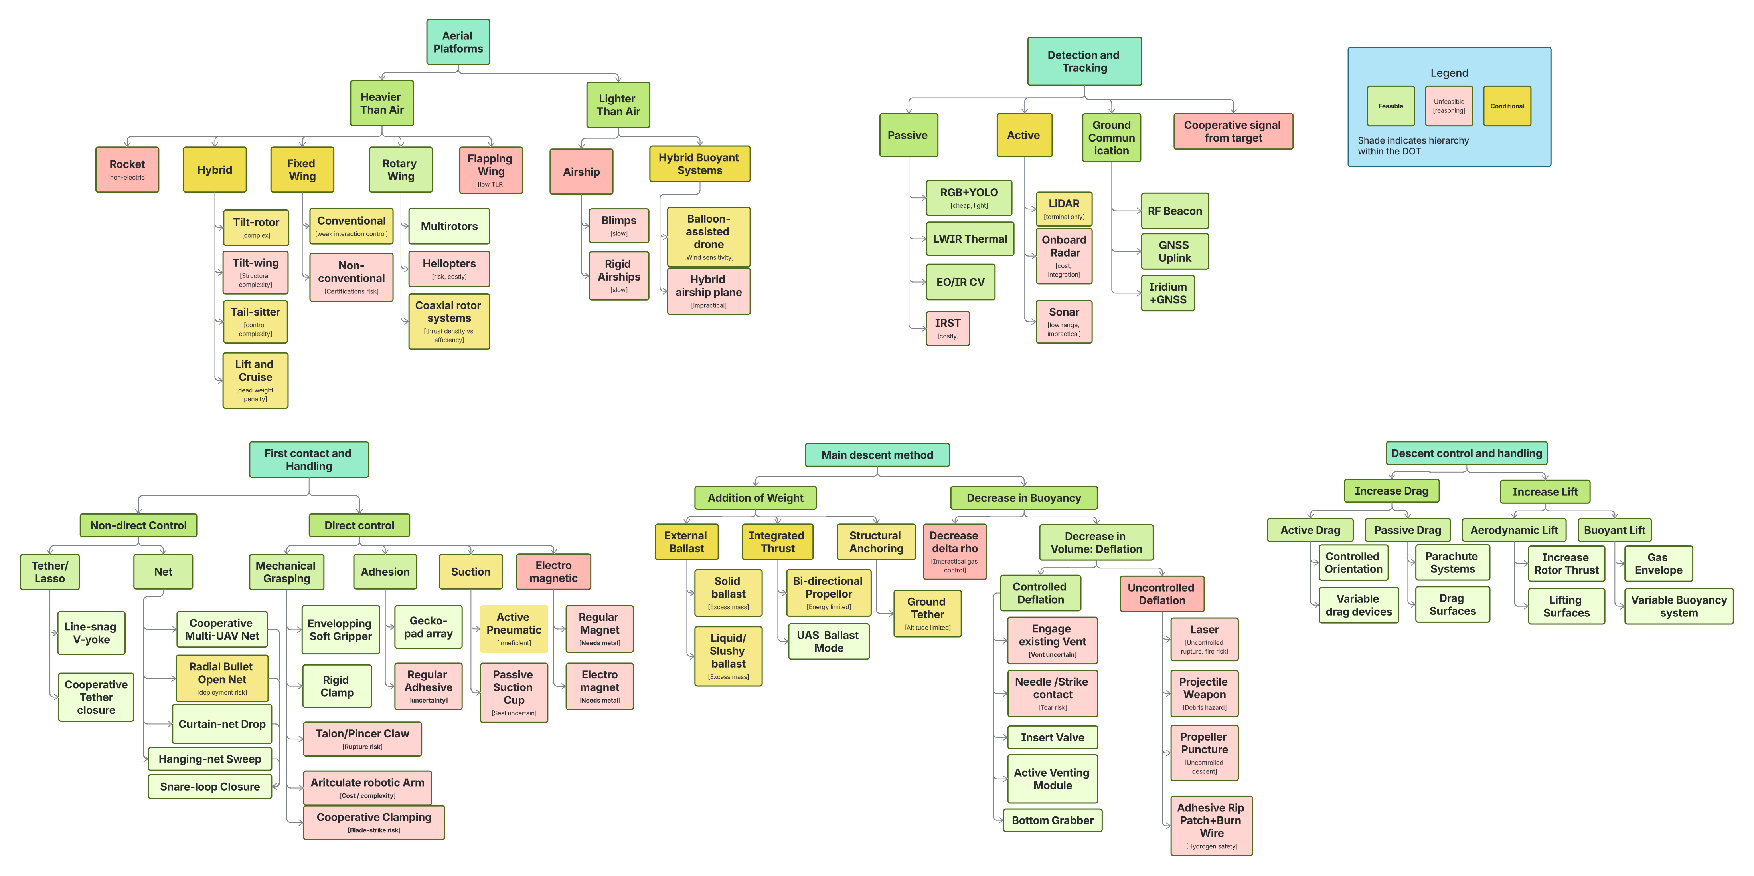
\includepdf[
    pages=-,
    templatesize={420mm}{297mm},
    fitpaper=true,
    scale=1.3,
    pagecommand={
        \label{sec:design-option-tree}
        \captionof{figure}{Design option tree for the BELLONA midterm concept generation process.}
        \label{fig:dot-midterm}
    },
]{figures/DOT_Midterm.pdf}


% \section{Overview of the Five Selected Concepts}

% The retained design-option-tree branches were combined into five complete mission concepts.
% Each concept combines an aerial platform, a balloon-interaction method, and a descent or
% recovery strategy. Table~\ref{tab:concept_overview_compact} provides the overview used as
% the starting point for the concept descriptions and trade-off.

% \begin{table}[H]
%     \centering
%     \small
%     \caption{Compact overview of the five concepts entering the trade-off.}
%     \label{tab:concept_overview_compact}
%     \begin{tabularx}{\textwidth}{@{}
% >{\raggedright\arraybackslash}p{0.035\textwidth}
% >{\raggedright\arraybackslash}p{0.12\textwidth}
% >{\raggedright\arraybackslash}p{0.40\textwidth}
% >{\raggedright\arraybackslash}X
% @{}}
%         \toprule
%         \textbf{ID} & \textbf{Concept} & \textbf{Core architecture} & \textbf{Recovery principle} \\
%         \midrule
%         A & Payload Fishing 
%         & Tail-sitter VTOL captures the suspended payload from below using an upward-launched net. 
%         & UAV weight and thrust pull the coupled system down, with parachute backup. \\

%         B & Pick and Drop 
%         & Carrier eVTOL deploys cooperative net drones and an intervention drone around the balloon-payload system. 
%         & Two-stage net containment, controlled deflation and guided parafoil descent. \\

%         C & Mechanical Clamping 
%         & Lift-and-cruise eVTOL secures the payload or attachment using deployable clamping beams. 
%         & UAV mass and directed thrust guide the coupled system to the recovery zone. \\

%         D & Cooperative Payload Net 
%         & Three multirotors suspend and close a shared net around the payload or lower flight train. 
%         & Added ballast and net hardware overcome free lift while the UAV team steers descent. \\

%         E & Kinetic Bolas 
%         & Hybrid UAV launches a weighted bolas line around the suspension line. 
%         & Tether reel-out, UAV weight and thrust guide the balloon-payload system downward. \\
%         \bottomrule
%     \end{tabularx}
% \end{table}





\section{Baseline Sizing}

All concepts are designed using a common baseline. Below, the method behind the descent profile and an initial estimation of MTOW is illustrated. Additionally, the cost will be estimated for each concept. These numbers will be reported as pure parts acquisition cost.
\subsection*{Descent Profile}

A critical design driver is the drone's ability to descend while dragging the balloon against sustained winds. At a static equilibrium altitude of 6~km, the balloon volume ($V$) is determined by the buoyancy requirement:

\begin{equation}
    W \cdot g = V \cdot (\rho_{atm} - \rho_{H_2}) \cdot g
\end{equation}

For the given parameters, $V = 87.68\text{ m}^3$, resulting in a radius $r = 2.75\text{ m}$ and a projected area $S = 23.87\text{ m}^2$. 

The drag force ($D$) is calculated using the drag coefficient for a sphere ($C_D = 0.47$) and a design wind speed of 13~m/s (derived from a 21~m/s gust and a 1.62 gust factor). Using the mean air density $\rho$ between sea level and 6~km:

\begin{equation}
    D = \frac{1}{2} \rho v^2 S C_D = \frac{1}{2} \left( \frac{1.225 + 0.66}{2} \right) \cdot 13^2 \cdot 23.87 \cdot 0.47 \approx 894.4\text{ N}
\end{equation}

%\begin{equation}
%    D = \frac{1}{2} \rho v^2 S C_D = \frac{1}{2}  0.66  \cdot 34^2 \cdot 23.87 \cdot 0.47 \approx 4280\text{ N}
%\end{equation}

\section{Common Mission Assumptions}
\label{sec:common_mission_assumptions}
All concepts have certain common operational assumptions
External cueing provides the initial balloon position, altitude, and drift estimate. The cue may
come from airport surveillance, mobile radar, visual observation, or another ground monitoring
source.
The ground station supervises launch, target handover, mission approval, abort decisions, and
recovery-zone coordination. A recovery crew retrieves the balloon, payload, and deployed
hardware after landing. The recovery zone is selected or updated during the mission using the
descent-start location, weather, and ground-risk constraints from Table 2.1.
All concepts must avoid pyrotechnic or explosive interaction, avoid uncontrolled balloon rupture,
and keep the post-contact balloon-payload system in a controlled state. Descent and recovery
estimates are used as concept-level comparison tools. Detailed flight dynamics, tether dynamics,
regulatory approval, and recovery-zone clearance remain verification items for later design
phases.




\subsection*{Power and Mass}
\label{sec:power_mass}

The vehicle mass is estimated using an iterative sizing loop that ensures the Maximum Take-Off Weight ($MTOW$) can support the energy requirements of the mission. The total mass is defined as:
\begin{equation}
    MTOW = m_{batt} + m_{struct} + m_{prop} + m_{fixed} + m_{margin}
\end{equation}
where $m_{struct}$ and $m_{prop}$ are modeled as fractions of the total weight ($f_{struct}$ and $f_{prop}$ respectively). 


The battery mass ($m_{batt}$) is derived from the total mission energy ($E_{total}$), specific energy density ($\rho_{batt}$), and an operational reserve ($R_{res}$):
\begin{equation}
    m_{batt} = \frac{E_{total}}{\rho_{batt} \cdot (1 - R_{res})}
\end{equation}
The total energy is the sum of the power consumed during each flight phase ($i$) multiplied by the phase duration ($t_i$):
\begin{equation}
    E_{total} = \sum P_i t_i = (P_{climb} t_{climb}) + (P_{hover} t_{hover}) + (P_{cruise} t_{cruise}) + (P_{descent} t_{descent})
\end{equation}
The power requirements for each phase are calculated as follows:
\begin{itemize}
    \item \textbf{Hover Power:} $P_{hover} = \frac{1}{\eta_{hover}} \sqrt{\frac{(MTOW \cdot g)^3}{2 \rho A}}$ \cite{Leishman2006}
    \item \textbf{Cruise Power:} $P_{cruise} = \frac{(\frac{1}{2} \rho V^2 S C_D) \cdot V}{\eta_{prop}}$
    \item \textbf{Climb Power:} $P_{climb} = \frac{MTOW \cdot g \cdot v_{climb}}{\eta_{climb}}$
    \item \textbf{Descent Power (Towing):} $P_{descent} = F_{drag, balloon} \cdot v_{wind}$
\end{itemize}

The final weight is calculated iteratively from the battery mass and
component mass fractions until the estimate converges.

% \section{Shared Descent-Rate Estimate}
% \label{sec:shared_descent_rate_estimate}

% Several concepts rely on applying additional downward force to the balloon after capture. To compare these concepts consistently, a shared first-order descent-rate estimate is used. The equivalent excess downward mass is defined as the remaining downward force after the balloon residual free lift has been overcome. At terminal descent, this excess downward force is balanced by the vertical drag of the balloon, approximated as a spherical bluff body:

% \begin{equation}
%     m_{\mathrm{excess}} g =
%     \frac{1}{2}\rho V_{\mathrm{des}}^2 S C_D
% \end{equation}

% Solving for the descent speed gives:

% \begin{equation}
%     V_{\mathrm{des}} =
%     \sqrt{
%     \frac{2m_{\mathrm{excess}}g}
%     {\rho S C_D}
%     }
%     \label{eq:shared_descent_velocity}
% \end{equation}

% where \(\rho\) is the air density, \(S\) is the projected balloon area, and \(C_D = 0.47\) is used as a first-order drag coefficient for a sphere. The estimate is evaluated at \(0.660~\mathrm{kg/m^3}\) at \(6~\mathrm{km}\) altitude and \(1.225~\mathrm{kg/m^3}\) near sea level. The descent time is estimated using the average of the two terminal speeds.

% \begin{table}[H]
% \centering
% \small
% \caption{Indicative terminal descent-rate and descent-time estimate after capture. \(m_{\mathrm{excess}}\) is the equivalent downward mass remaining after the balloon residual free lift has been overcome.}
% \label{tab:shared_descent_time_estimate}
% \setlength{\tabcolsep}{6pt}
% \renewcommand{\arraystretch}{1.15}
% \begin{tabular}{ccccc}
% \toprule
% \textbf{Balloon diameter} 
% & \textbf{Excess mass} 
% & \textbf{Rate at 6 km} 
% & \textbf{Rate at ground} 
% & \textbf{Descent time} \\
% \midrule
% \(2~\mathrm{m}\) & \(10~\mathrm{kg}\) & \(14.2~\mathrm{m/s}\) & \(10.4~\mathrm{m/s}\) & \(8.1~\mathrm{min}\) \\
% \(2~\mathrm{m}\) & \(25~\mathrm{kg}\) & \(22.4~\mathrm{m/s}\) & \(16.5~\mathrm{m/s}\) & \(5.1~\mathrm{min}\) \\
% \(2~\mathrm{m}\) & \(50~\mathrm{kg}\) & \(31.7~\mathrm{m/s}\) & \(23.3~\mathrm{m/s}\) & \(3.6~\mathrm{min}\) \\
% \midrule
% \(6~\mathrm{m}\) & \(10~\mathrm{kg}\) & \(4.7~\mathrm{m/s}\) & \(3.5~\mathrm{m/s}\) & \(24.4~\mathrm{min}\) \\
% \(6~\mathrm{m}\) & \(25~\mathrm{kg}\) & \(7.5~\mathrm{m/s}\) & \(5.5~\mathrm{m/s}\) & \(15.4~\mathrm{min}\) \\
% \(6~\mathrm{m}\) & \(50~\mathrm{kg}\) & \(10.6~\mathrm{m/s}\) & \(7.8~\mathrm{m/s}\) & \(10.9~\mathrm{min}\) \\
% \bottomrule
% \end{tabular}
% \end{table}

% This estimate only covers vertical descent due to excess downward force and balloon drag. It excludes wind drift, steering, tether dynamics, payload drag, parafoil effects and envelope deformation. 
 


\section{Concept A: Vertical Net Launch}
\label{sec:concept_A}

Concept A captures the suspended payload from below using an
upward-launched net, then tows the balloon-payload system toward the
selected recovery zone. A tail-sitter VTOL provides efficient transit
and hover authority for the net launch. The mission sequence is shown
in \autoref{fig:CAOoO}, with the aerial platform as shown in \autoref{fig:CAOoO}

\begin{figure}[H]
    \centering
    % Left Subfigure (Operational Sequence)
    \begin{subfigure}[b]{0.58\linewidth}
        \centering
        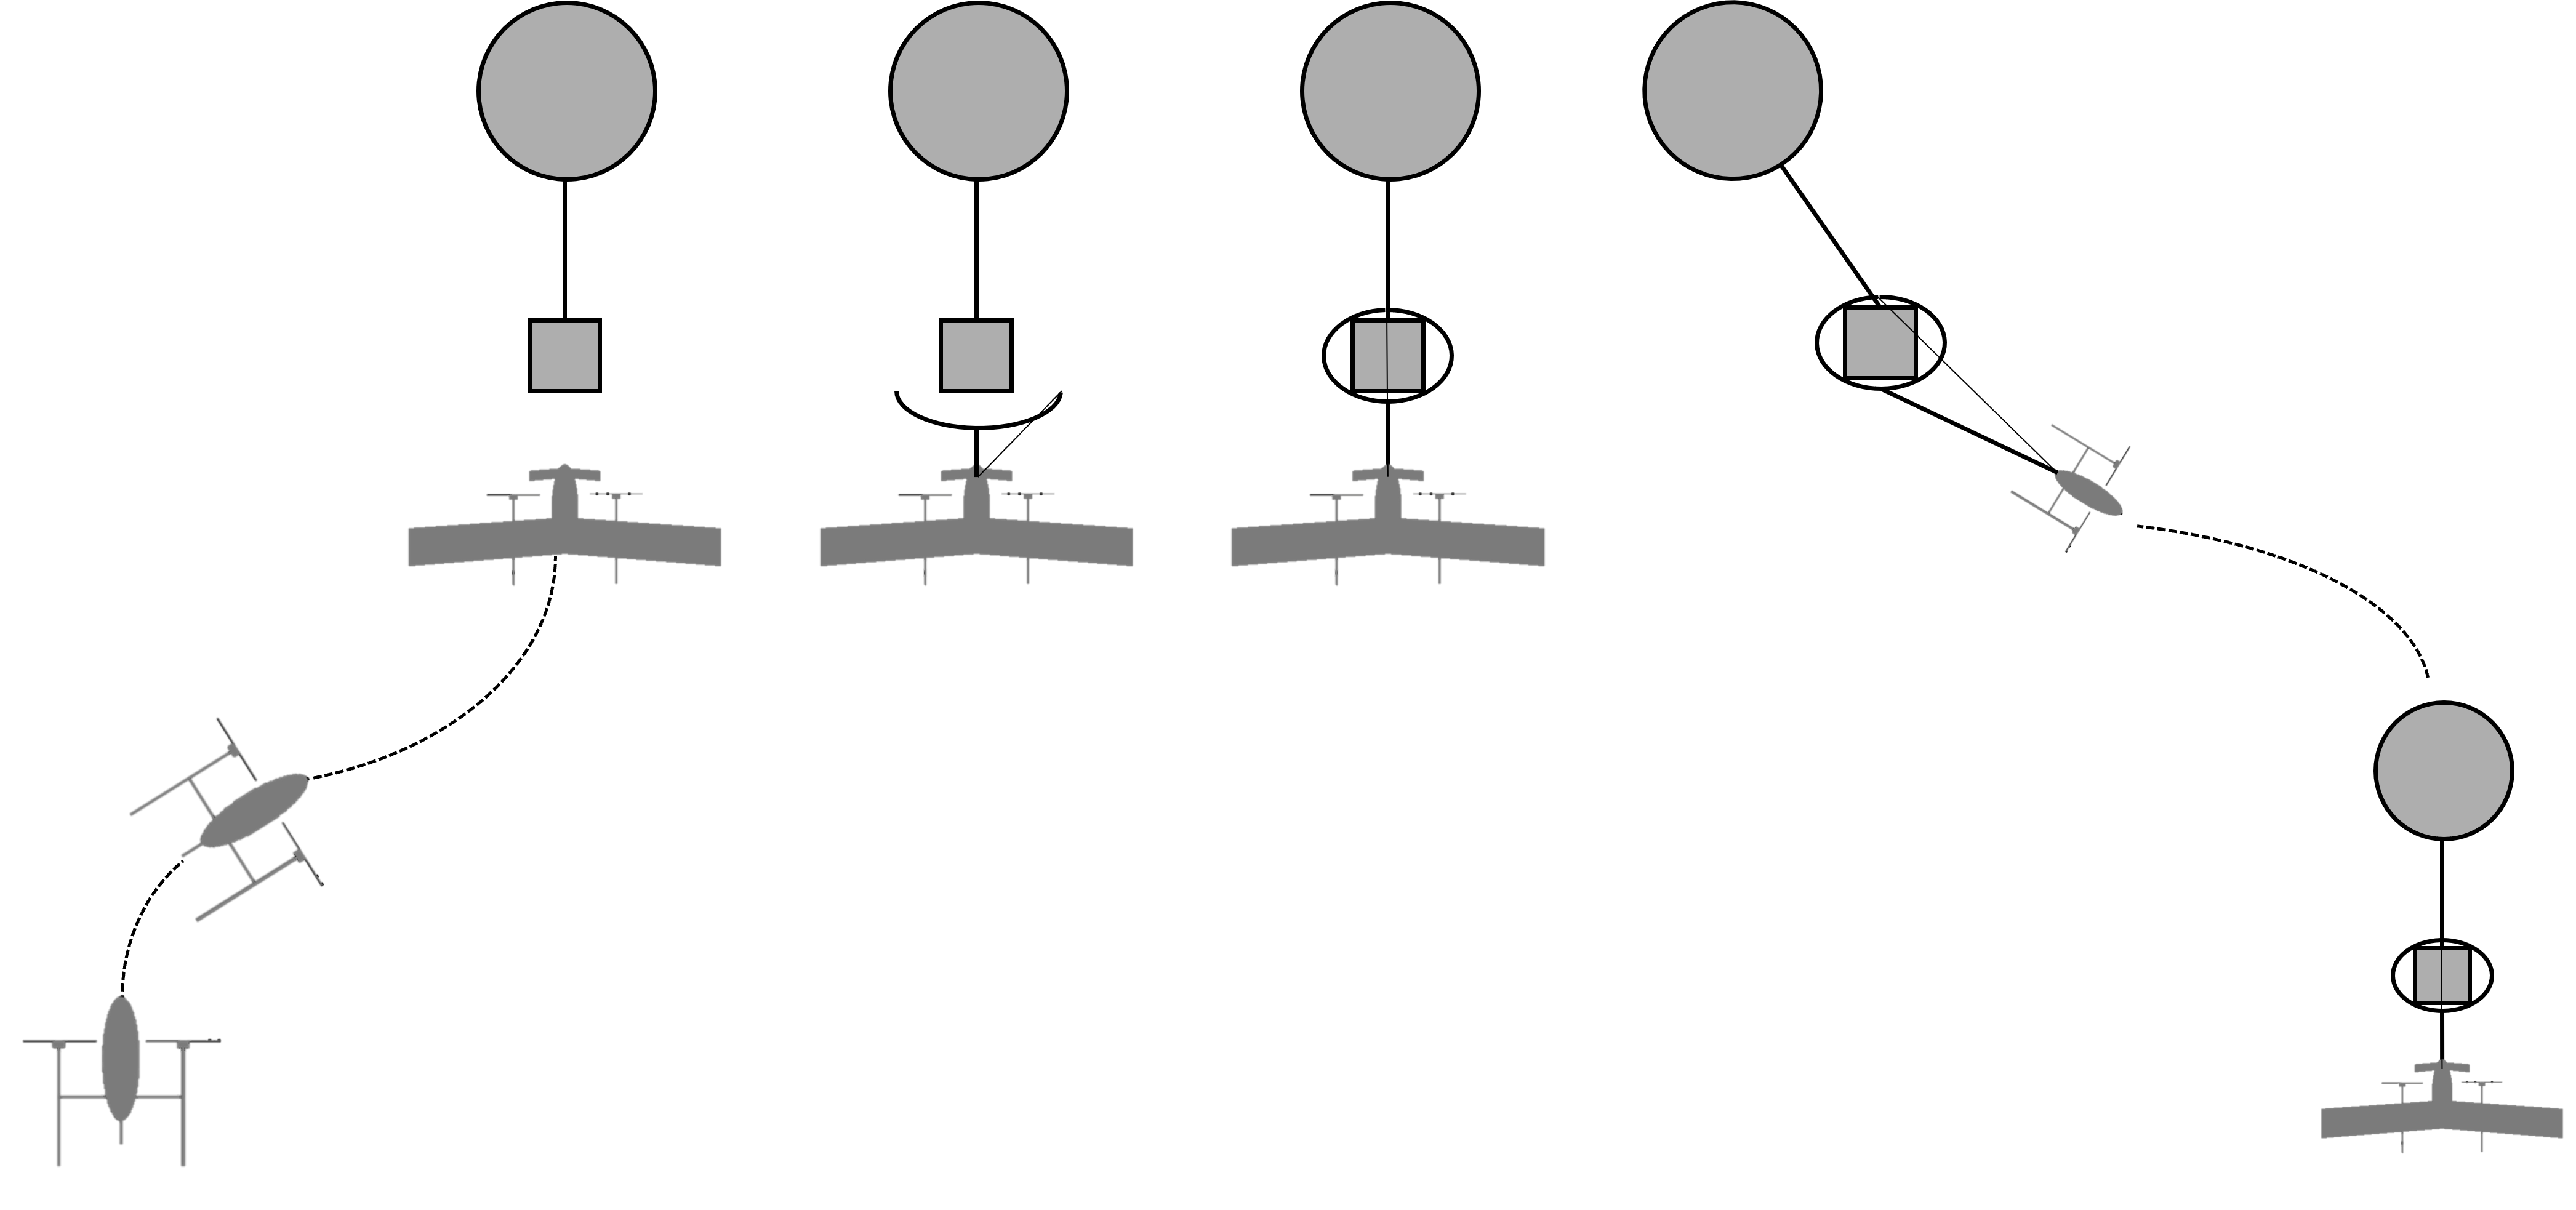
\includegraphics[width=\linewidth]{figures/Concepts/Fishing - Order of Operations.png}
        \caption{Operational Sequence}
        \label{fig:CAOoO}
    \end{subfigure}
    \hfill % This pushes the two images to the outer edges
    % Right Subfigure (Conceptual Layout)
    \begin{subfigure}[b]{0.38\linewidth}
        \centering
        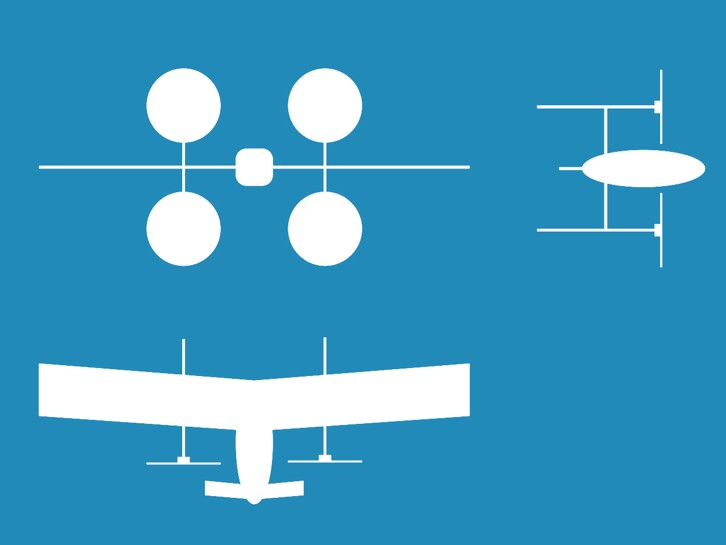
\includegraphics[width=\linewidth]{figures/Concepts/Fishing Design.jpg}
        \caption{Conceptual Tail-sitter Layout}
        \label{fig:ConceptADesign}
    \end{subfigure}
    
    % Main overarching caption and label
    \caption{Design and operational overview for Concept A.}
    \label{fig:ConceptAOverview}
\end{figure}


\subsection{System Architecture}
\subsubsection{Aerial Platform}
The proposed aerial platform is a four-propeller tail-sitter UAV. The configuration combines wing-borne cruise with vertical take-off, landing, and hover below the
payload. This is the key advantage over a pure multirotor, which would
be simpler during capture but less efficient during climb and transit,
and over a conventional fixed-wing aircraft, which cannot hold position
below the payload. The UAV uses a canard layout. The net gun and sensor
suite are mounted in the nose, while the reel and tether are placed near
the centre of mass to reduce towing moments.



\subsubsection{Sensing and Tracking}
\label{subsec:Sensing_tracking}
Concept A uses the common external-cueing architecture in \autoref{sec:common_mission_assumptions}. For terminal tracking,
the proposed onboard sensors include a long-wave infrared camera and a
short-range mmWave radar with multiple antennas for improved angular
accuracy \cite{Soumya2023RecentReview}. The onboard computer estimates
the payload-relative position for hover below the target. After capture,
tether-tension sensing monitors the load path.

\subsubsection{Balloon Interaction Mechanism}
The UAV hovers below the payload and launches a \(10\times10~\mathrm{m}\)
UHMWPE net using a compact net launcher, similar to the example in
\autoref{fig:netlauncher}. Corner weights spread the net during launch
and help it wrap around the payload. A tether connects the net to the
UAV and drives a pouch-closure line around the net edge.

After launch, the UAV transitions toward towing flight while the onboard
reel controls tether tension. Pulling the tether closes the net around
the payload and establishes the mechanical link for descent.

\begin{figure}[H]
    \centering
    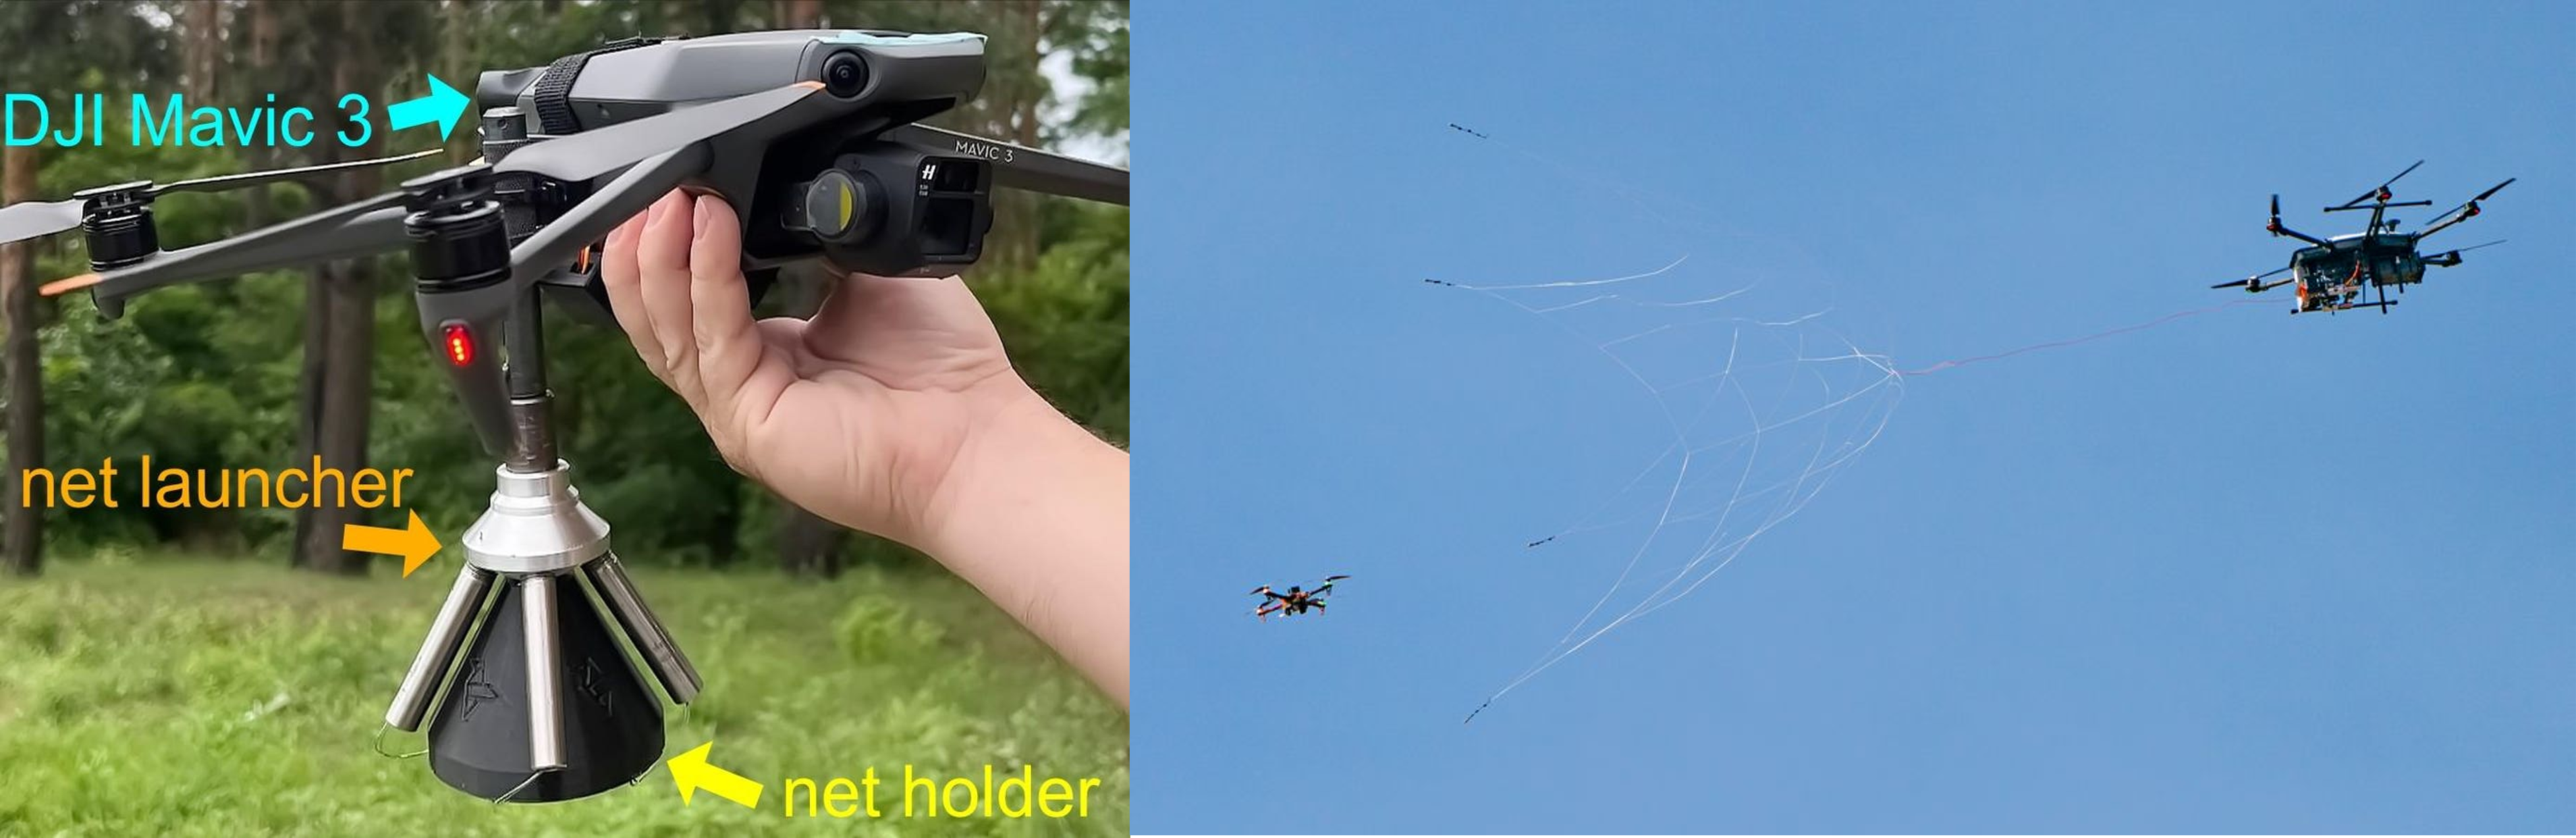
\includegraphics[width=0.7\linewidth]{figures/Concepts/Net_Launcher.png}
    \caption{Examples of UAV-based Net Launchers \cite{Hambling2024Webslingers2,Widdows2026NetCaptureWorldCup2}}
    \label{fig:netlauncher}
\end{figure}

As an additional safety feature, the tether system includes an emergency breakaway function. If the balloon ruptures or the balloon tether fails, the tether separates from the UAV. A small parachute attached to the released tether then deploys and slows the descent of the payload-net system. This prevents unsafe descent of the entire system.

\subsubsection{Descent Initiation}
The UAV finishes its transition to horizontal flight and begins its descent towards the designated recovery location. Descent speed is managed to minimize risk of the balloon envelope rupturing or otherwise damaging the payload, while ensuring that the airspace hazard is promptly removed.

\subsubsection{Descent Management and Recovery}
The balloon is pulled downwards with a combination of propulsive thrust and the UAV weight. A continuous datalink reports target updates and tether-load status during towing. Shortly before landing in a designated recovery zone, the UAV transitions to hover and sets down while keeping the captured payload-net system restrained. After touchdown, the \(50~\mathrm{kg}\) UAV mass provides a passive anchoring margin against residual free lift until the recovery crew arrives.




\subsection{Mass, Cost, and Complexity Estimate}

The mass and cost estimate is based on a 50 kg tail-sitter UAV carrying a net launcher, sensor package, tether reel, battery system, and propulsion system. The capture hardware is relatively light compared with the propulsion and energy storage systems. A breakdown of the cost and mass budgets can be found in \autoref{tab:budgetsA}.

\begin{table}[H]
\centering
\caption{Mass and Cost Estimates for Option A}
\label{tab:budgetsA}{%
\begin{tabular}{lll}
\hline
\textbf{Part}                                   & \textbf{Mass [kg]} & \textbf{Cost [EUR]} \\ \hline
Net (incl. Net, Corner Weights, and Tether)     & 2                      & 150                   \\
Net Gun                                         & 2                      & 450                   \\
Sensors (incl. Cameras, mmWave Radar, and Telemetry)  & 1                      & 1500                  \\
Flight Controller                               & 0.5                    & 500                   \\
Power Source (incl. Batteries and Cabling)      & 18.2                   & 2000                  \\
Propulsion (incl. Motors, Propellers, and ESCs) & 12                     & 5000                  \\
Airframe                                        & 10                     & 3000                  \\
Miscellaneous                                   & 4.3                    & 1000                  \\
\textbf{Total}                                  & \textbf{50}            & \textbf{13 600}       \\ \hline
\end{tabular}%
}
\end{table}

More details on the aerial system can be found in \autoref{tab:SpecsA}.



\begin{table}[H]
\centering
\caption{Concept A: Specifications of Aerial System}
\label{tab:SpecsA}
\begin{tabular}{cccccc}
\hline
\textbf{No. Rotors} & \textbf{Max Thrust / Rotor} & $\mathbf{CL_{cruise}}$ & \textbf{Wing Area} & \textbf{Battery Capacity} & $\mathbf{V_{cruise}}$ \\ \hline
4 & 35~kg & 0.5 & $7.4~\mathrm{m^2}$ & 3.28~kWh (11.8~MJ) & 20~m/s \\ \hline
\end{tabular}
\end{table}

\subsection{Risks and Uncertainties}
The main risk is failed net capture. Payload swing or an irregular
payload shape can cause the net to miss or fall back toward the UAV.
A large net aperture reduces this risk.

Clouds and low-light conditions can reduce tracking performance. The
mixed EO/IR, radar, and ground-cueing architecture provides sensing
redundancy for terminal approach.

Another important risk is sudden loss of balloon lift. If the balloon ruptures or the payload enters free fall while attached to the UAV, the tether load could destabilize the aircraft. The backup parachute reduces this risk by separating the UAV from the falling payload and slowing the payload descent.

Finally, the tail-sitter transition while carrying a tethered load is a significant control challenge. The concept therefore depends strongly on reliable hover tracking, tether-load management, and flight-control testing with representative loads.


\section{Concept B: Pick and Drop}
 

Concept B uses a fixed-wing carrier eVTOL to deliver three net-carrying
multirotors and one intervention multirotor to the interception region.
The net carriers form a capture volume below the balloon-payload system.
The intervention drone clamps the balloon tether near the load ring, and
an electric winch draws the balloon and payload into the two-stage net.
After capture, the intervention drone applies an adhesive rip-patch to
the envelope to initiate deflation. The closed net contains the target
during controlled deflation and guided parafoil descent.

\subsection{System Architecture}
\label{subsec:concept_B_architecture}

\subsubsection{Aerial Platform}
The capture team consists of three heavy-lift multirotor net carriers
with a per-vehicle MTOW of \(8.5~\mathrm{kg}\), plus a smaller
intervention drone for tether engagement and envelope intervention. The
four vehicles are packed inside a fixed-wing eVTOL carrier with an
\(81~\mathrm{kg}\) launch MTOW. The carrier performs the climb and
transit leg; the multirotors provide local hover authority during
capture.


\subsubsection{Sensing and Tracking}
\label{subsubsec:conceptB_sensing_tracking}

Concept B uses the common external cue for carrier navigation and then
adds distributed local sensing. The carrier refines the target state
using GNSS/INS, barometric altitude, airspeed sensing, and a gimballed
RGB/IR camera. After deployment, the net carriers use GNSS, IMU,
barometer, short-range communication, and upward-looking cameras to hold
position below the target. Load cells, tether-tension sensors, and winch
position sensors indicate whether the net is open, closing, loaded, or
secured. The intervention drone uses a forward camera, short-range depth
sensing, a clamp contact switch, and patch contact-force sensing for
tether engagement and controlled deflation.

 
\begin{figure}[H]
    \centering
    \resizebox{0.4\textwidth}{!}{%
    \begin{tikzpicture}[x=1pt,y=-1pt,line cap=round,line join=round]
        \fill[white] (0,0) rectangle (520,520);

        \begin{scope}
            \clip (260,265) circle (218);
            \foreach \y in {145,185,225,265,305,345,385}
                \draw[gray!45,dash pattern=on 5pt off 6pt,line width=0.5pt] (42,\y) -- (478,\y);
            \foreach \x in {140,180,220,260,300,340,380}
                \draw[gray!45,dash pattern=on 5pt off 6pt,line width=0.5pt] (\x,42) -- (\x,488);
        \end{scope}

        \draw[gray!55,dash pattern=on 6pt off 4pt,line width=1pt] (260,265) circle (218);
        \draw[blue!65!black,dash pattern=on 12pt off 5pt,line width=3pt] (260,265) circle (218);
        \draw[fill=gray!8,draw=orange!75!red,line width=2.5pt] (260,265) circle (44);
        \draw[orange!75!red,dash pattern=on 6pt off 3pt,line width=2pt] (260,265) circle (50);
        \draw[orange!75!red,dash pattern=on 6pt off 3pt,line width=2pt] (260,215) -- (260,162);
        \draw[orange!75!red,line width=2pt] (260,155) circle (7);
        \fill[orange!75!red] (260,155) circle (3);

        \node[font=\bfseries\scriptsize,text=orange!45!black] at (260,260) {inner circle};
        \node[font=\scriptsize,text=orange!45!black] at (260,276) {\(\varnothing \approx 1.94\,\mathrm{m}\)};

        \foreach \x/\y/\name/\lx/\ly/\ax/\ay/\bx/\by in {
            260/41/D1/260/29/260/49/260/47,
            71/382/D2/71/370/85/382/99/374,
            449/382/D3/449/370/435/382/421/374
        }{
            \draw[fill=gray!15,draw=gray!65,line width=1.2pt,rounded corners=3pt] (\x-14,\y-8) rectangle (\x+14,\y+8);
            \foreach \dx/\dy in {-11/-5,11/-5,-11/5,11/5}
                \draw[gray!65,line width=1pt] (\x+\dx,\y+\dy) circle (3.5);
            \node[font=\bfseries\scriptsize,text=gray!55!black] at (\lx,\ly) {\name};
            \draw[gray!65,line width=1pt] (\ax,\ay) -- (\bx,\by);
        }

        \draw[gray!70,dash pattern=on 3pt off 3pt,line width=0.8pt] (260,290) -- (478,290);
        \draw[gray!70,line width=0.8pt] (260,285) -- (260,295);
        \draw[gray!70,line width=0.8pt] (478,285) -- (478,295);
        \node[font=\scriptsize,text=gray!55!black] at (369,307) {\(r=12\,\mathrm{m}\)};

        \draw[gray!70,dash pattern=on 3pt off 3pt,line width=0.8pt] (260,290) -- (304,290);
        \node[font=\scriptsize,text=orange!45!black] at (312,307) {\(r=0.97\,\mathrm{m}\)};

        \node[font=\bfseries\scriptsize,text=blue!55!black] at (260,500) {outer lace, \(\varnothing\approx24\,\mathrm{m}\), length \(\approx75\,\mathrm{m}\)};
        \node[anchor=west,font=\bfseries\scriptsize,text=orange!45!black] at (12,206) {inner lace};
        \node[anchor=west,font=\scriptsize,text=orange!45!black] at (12,220) {threads inner circle};
        \draw[-{Latex[length=5pt]},orange!75!red,line width=0.8pt] (95,213) -- (207,258);
        \node[anchor=west,font=\scriptsize,text=orange!45!black] at (270,152) {ties to balloon base};
        \node[anchor=west,font=\scriptsize,text=orange!45!black] at (270,164) {when closed};
    \end{tikzpicture}}
    \caption{Top-down flat layout view of the balloon net.}
    \label{fig:net_layout}
\end{figure}


\subsubsection{Balloon Interaction Mechanism}
A shared two-stage net displayed in \autoref{fig:net_layout} (8~m diameter aperture, 50 m$^2$) is suspended horizontally between the three net carriers via burn-wire releasable suspension cables. The intervention drone delivers a mechanical clamp to the upper end of the balloon tether near the load ring; the clamp is connected through 35 m of 2 mm Dyneema leash to an electric winch on the net rim. The inner-stage drawline cinches around the payload at the top, before the distance between the crate and balloon is eliminated, and later the outer-stage drawline cinches around the balloon.


\subsubsection{Descent Initiation}
Descent is initiated by controlled deflation. An adhesive rip-patch (100 g, 10$\times$10 cm contact area) with embedded NiChrome burn-wire is applied through the upper net stage. The burn-wire softens the envelope material, and the intervention drone, held at 5 m standoff and still connected to the patch by a wire, pulls the patch free, opening an aperture of 0.05 m$^2$. Effusion proceeds at 0.07 kg/s for a $\varnothing$6~m helium balloon at altitude, giving a buoyancy half-life of 80 s. The envelope remains contained inside the closed net throughout deflation.

\subsubsection{Descent Management and Recovery}
A guided ram-air parafoil with an Autonomous Guidance Unit (AGU), sized for 60 kg descent mass at 5 m/s, is packed in a deployment bag tied the net rim, placed on the bottom and on the exterior of the inner payload ring so its weight distributes evenly across the three drones during transit. A spring ejection system ensures immediate canopy exposure regardless of bundle orientation; a pilot chute then extracts the main canopy, which inflates in 3 s. After bundle release, the capture drones, intervention drone, and carrier return autonomously to the ground station.



\subsection{Preliminary Mass, Power and Cost Estimate}

A compact first-order sizing was performed for the split-mission Concept~B architecture. The carrier transports the three-drone capture team to $6000~\mathrm{m}$ altitude and $6000~\mathrm{m}$ ground range using wing-borne climbing cruise. The net-carrying rotorcraft are sized only for the local capture hover and powered descent after release. The sizing assumes $265~\mathrm{Wh/kg}$ batteries with $20\%$ reserve, rotor disk loading of $15~\mathrm{kg/m^2}$, rotor figure of merit $0.70$, and carrier $L/D=12$. The vehicle costs are order-of-magnitude component-scaled estimates, while payload-hardware costs are retained from the existing concept estimate.

\begin{table}[H]
\centering
\footnotesize % Slightly smaller font to guarantee zero overrun
\setlength{\tabcolsep}{3.5pt} % Trims padding between columns

% --- LEFT TABLE ---
\begin{minipage}[t]{0.48\textwidth}
\centering
\caption{Hybrid carrier mass, power and cost estimate.}
\label{tab:conceptB_carrier_compact}
\begin{tabular}{lrr}
\hline
\textbf{Item} & \textbf{Mass/Power} & \textbf{Cost [EUR]} \\
\hline
Structure & $20.33~\mathrm{kg}$ & $6\,100$ \\
Propulsion & $16.26~\mathrm{kg}$ & $6\,800$ \\
Avionics \& control & $4.07~\mathrm{kg}$ & $5\,400$ \\
Battery & $13.17~\mathrm{kg}$ & $1\,450$ \\
Mass margin & $2.03~\mathrm{kg}$ & $500$ \\
Delivered payload & $25.45~\mathrm{kg}$ & -- \\
\hline
\textbf{MTOW / Vehicle Cost} & \textbf{$81.31~\mathrm{kg}$} & \textbf{20k--25k} \\
\hline
Climbing-cruise power & $12.05~\mathrm{kW}$ & -- \\
Descent power & $2.48~\mathrm{kW}$ & -- \\
Usable battery energy & $2.79~\mathrm{kWh}$ & -- \\
\hline
\end{tabular}
\end{minipage}
\hfill % Pushes the tables to the absolute left and right boundaries
% --- RIGHT TABLE ---
\begin{minipage}[t]{0.48\textwidth}
\centering
\caption{Single net-carrying rotorcraft estimate (3 identical units used).}
\label{tab:conceptB_rotorcraft_compact}
\begin{tabular}{lrr}
\hline
\textbf{Item} & \textbf{Mass/Power} & \textbf{Cost [EUR]} \\
\hline
Structure & $1.70~\mathrm{kg}$ & $500$ \\
Propulsion & $1.53~\mathrm{kg}$ & $650$ \\
Avionics \& control & $0.42~\mathrm{kg}$ & $550$ \\
Battery & $0.99~\mathrm{kg}$ & $100$ \\
Mass margin & $0.18~\mathrm{kg}$ & $50$ \\
Capture hardware & $3.67~\mathrm{kg}$ & -- \\
\hline
\textbf{MTOW / Vehicle Cost} & \textbf{$8.48~\mathrm{kg}$} & \textbf{$1\,800-2\,200$} \\
\hline
Hover power & $1.26~\mathrm{kW}$ & -- \\
Powered-descent power & $0.38~\mathrm{kW}$ & -- \\
Energy requirement & $209~\mathrm{Wh}$ & -- \\
\hline
\end{tabular}
\end{minipage}
\end{table}




{
\small
\setlength{\LTleft}{0pt}
\setlength{\LTright}{0pt}
\setlength{\tabcolsep}{4pt}

\begin{longtable}{@{}
>{\raggedright\arraybackslash}p{0.30\textwidth}
>{\raggedleft\arraybackslash}p{0.05\textwidth}
>{\raggedleft\arraybackslash}p{0.15\textwidth}
>{\raggedright\arraybackslash}p{0.45\textwidth}
@{}}
\caption{Payload and capture-hardware mass and cost estimate. Values not produced by the sizing code are retained from the concept hardware estimate.}
\label{tab:conceptB_payload_compact} \\
\hline
\textbf{Element} & \textbf{Mass [kg]} & \textbf{Cost [EUR]} & \textbf{Note} \\
\hline
\endfirsthead

\hline
\textbf{Element} & \textbf{Mass [kg]} & \textbf{Cost [EUR]} & \textbf{Note} \\
\hline
\endhead

\hline
\endfoot

Capture net & $2.0$ & $2\,000-3\,000$ & HMPE/Dyneema mesh with reinforced rim \\
Main shortening/winch mechanism & $1.3$ & $1\,000-1\,500$ & Motor, drum, frame, ESC and Dyneema leash \\
Cinch drawline mechanism & $0.4$ & $200-400$ & Secondary net-closure mechanism \\
Guided parafoil with AGU & $5.0$ & $8\,000-15\,000$ & Sized for $60~\mathrm{kg}$ descent mass at $5~\mathrm{m/s}$ \\
Rip-patch and burn-wire kit & $0.5$ & $200-400$ & Controlled balloon deflation device \\
Net-to-drone release hardware & $0.3$ & $150-300$ & Three burn-wire cable cutters \\
Auxiliary intervention drone & $1.5$ & $1\,200-1\,500$ & Tether engagement and patch application \\
\textbf{Payload hardware subtotal} & \textbf{$11.0$} & \textbf{$12\,750-22\,100$} & Carried by the three net-carrying rotorcraft \\

\end{longtable}
}
The carrier reaches the release point after approximately $600~\mathrm{s}$, matching the $10~\mathrm{min}$ reference interception time. Including the $300~\mathrm{s}$ capture hover phase, capture completion occurs after approximately $900~\mathrm{s}$. The total hardware acquisition estimate for Concept~B is therefore approximately $38\,000-54\,000$ EUR.



\subsection{Risks and Uncertainties}
The main recovery risk is parafoil ground reach. With a representative
minimum glide ratio of 3:1, release from \(6~\mathrm{km}\) altitude gives
an approximate \(18~\mathrm{km}\) landing-radius requirement. This limits
recovery-zone selection unless additional mass and control authority are
allocated to the descent system.

Concept B also has many mission-critical stage transitions: carrier
release, net formation, tether clamp engagement, winch closure,
controlled deflation, parafoil deployment, and bundle release. A failure
in any of these steps can prevent mission completion.



\section{Concept C: Mechanical Clamping}
Concept C uses a lift-and-cruise eVTOL UAV, shown in
\autoref{fig:liftcruiseconcept}, to intercept the target and hold
position directly below the payload. The platform deploys two aluminium
clamping beams that extend outward, rotate upward, and secure the
payload or lower attachment without contacting the balloon envelope.
After capture, the UAV uses its mass and directed thrust to initiate and
stabilise a controlled descent toward the recovery zone.

\subsection{System Architecture}
\noindent 

\begin{figure}[htbp]
     \centering
     % Right Image: The Drone Concept
     \begin{subfigure}[b]{0.56\textwidth}
    
         \centering
         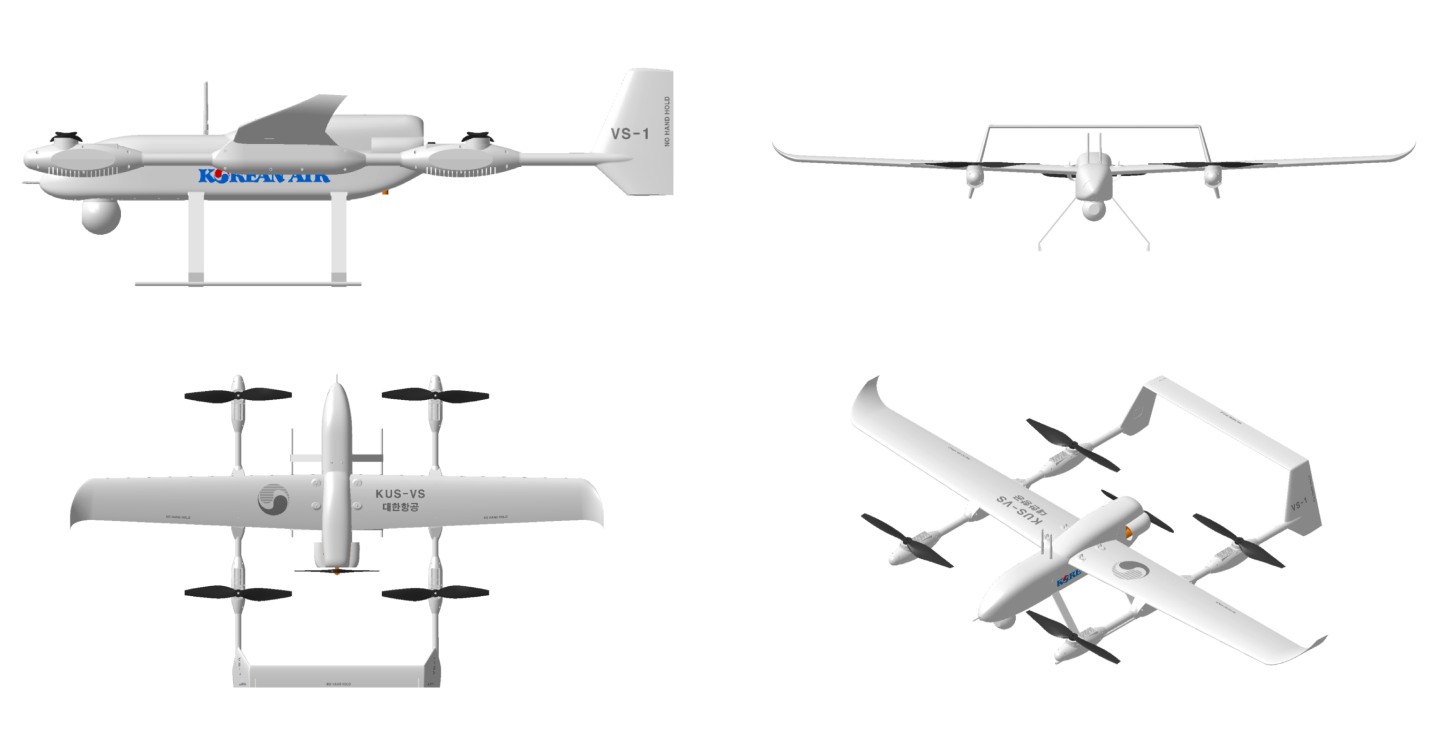
\includegraphics[width=\textwidth]{figures/Drone_concept.png}
          
         \caption{Integrated Lift \& Cruise Concept \cite{KoreanAirKoreanAerospace}}
         \label{fig:liftcruiseconcept}
     \end{subfigure}
     \hfill
     % Left Image: The Mechanism
     \begin{subfigure}[b]{0.32\textwidth}
         \centering
         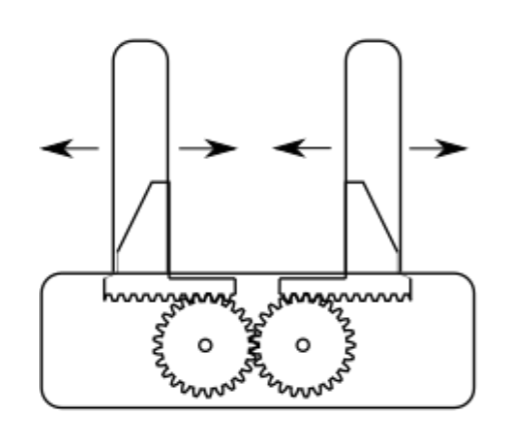
\includegraphics[width=\textwidth]{figures/Clamp_report.png}
         \caption{Linear Clamping Mechanism \cite{Correll2022IntroductionRobots}}
         \label{fig:clamping_mechanism}
     \end{subfigure}
     
     \label{fig:drone_design}
\end{figure}


\subsubsection{Aerial Platform}
Concept C requires a platform that can hold position beneath the payload while carrying the clamping beams and reacting the contact loads introduced during closure. A lift-and-cruise configuration is retained because it combines efficient transit to the intercept region with hover authority during the final payload approach and controlled descent.

The platform selection follows the Baseline Report screening
\cite{Group222026DSEReport}. Fixed-wing aircraft lack the hover
authority required for clamp closure, while tilt-rotor and tail-sitter
solutions add mechanical and control complexity. A lift-and-cruise UAV
therefore gives the best balance between transit efficiency and terminal
hover control for this concept.
\subsubsection{Sensing and Tracking}
Concept C uses the common external-cueing and terminal-sensing approach
from Section~\ref{sec:common_mission_assumptions}. Its concept-specific
sensing challenge is stable hover below the payload during clamp
deployment. Preliminary sizing assumes a forward-facing nose sensor
suite that supports sub-metre relative positioning during the final
approach.


\subsubsection{Balloon Interaction Mechanism}
The interaction mechanism avoids direct attachment to the balloon
envelope because uncontrolled perforation would reduce controllability.
It instead targets the payload or lower attachment region. The Baseline
Report identifies large variation in payload geometry, securing ropes,
and attachment angles \cite{Group222026DSEReport}; these variations can
increase rotor-strike risk and make point-contact mechanisms unreliable.
Suction, adhesion, and local soft-gripper options are therefore weak for
modified or irregular payloads. A beam clamp that captures the full
payload gives the most adaptable mechanical constraint for this concept.





\subsubsection{Descent Initiation}

After the payload is secured, the UAV lowers its vertical thrust so that
part of its weight is transferred through the clamp into the
balloon-payload system. This added downward load overcomes residual free
lift and starts the descent.

\subsubsection{Descent Management and Recovery}

During descent, the UAV remains connected to the balloon-payload system
through the clamp. Its directed thrusters regulate descent rate, provide
lateral control, and damp payload swing until touchdown in the recovery
zone. After bundle release, the UAV returns autonomously to the ground
station.


\subsection{Mass, Cost, and Complexity Estimate}

The first-order clamping estimate is based on the mechanism layout and
the loads expected during capture and descent. The clamp relies on
friction between the vertical arms and the payload. To limit loads in
the balloon ropes, the preliminary descent case uses an equivalent
\(50~\mathrm{kg}\) ballast effect from reduced UAV lift, which is
consistent with descent from \(6000~\mathrm{m}\) in less than
20 minutes. This load case keeps the rope safety factor near the
2.25 value used in relevant certification guidance
\cite{EASA2009EuropeanCS-31HB}.

The resulting vertical load is \(245~\mathrm{N}\) per clamping arm. For
Aluminium 6061-T6 contact with conservative compliant pads, a static
friction coefficient of \(0.3\) is assumed. The required normal force is
therefore \(245/0.3=817~\mathrm{N}\). Balloon drag adds
\(894.4~\mathrm{N}\) to the critical arm. The free-body diagram for this
arm is shown in \autoref{fig:FBD}.

\begin{figure}[h!]
    \centering
        \resizebox{0.6\textwidth}{!}{%
        \documentclass[tikz,border=10pt]{standalone}
\usetikzlibrary{arrows.meta, calc, patterns}

\begin{document}
\begin{tikzpicture}[
    force/.style={- {Stealth[scale=1.2]}, red, thick},
    reaction/.style={- {Stealth[scale=1.2]}, blue!70!black, thick},
    beam/.style={draw=black, fill=gray!15, thick},
    joint/.style={circle, draw=black, fill=white, inner sep=2pt},
    ext/.style={gray, thin},
    dim/.style={<->, >=Stealth, gray, thin}
]

    % --- Parameters ---
    \def\L{6}           % Visual length
    \def\width{0.4}     % Beam thickness
    \def\loadL{4.5}     % Length of the distributed load
    \def\arrowgap{0.6}  % Number of arrows in the load

    % --- Coordinates ---
    \coordinate (Shoulder) at (0,0);
    \coordinate (Elbow) at (-\L, 0);
    \coordinate (Wrist) at (-\L, \L);

    % --- Draw Support (Fixed Shoulder) ---
    \draw[pattern=north east lines, draw=black] (0,-0.6) rectangle (0.6,0.6);
    \draw[ultra thick] (0,-0.6) -- (0,0.6);

    % --- Draw Beams ---
    \draw[beam] (-\L, -\width/2) rectangle (0, \width/2); % Beam 1
    \draw[beam] ({-\L-\width/2}, 0) rectangle ({-\L+\width/2}, \L); % Beam 2

    % --- Dimensioning for Beam 1 (Horizontal) ---
    \def\offH{-1} % Offset below the beam
    \draw[ext] (-\L, -\width/2) -- (-\L, \offH - 0.2); % Left extension
    \draw[ext] (0, -\width/2) -- (0, \offH - 0.2);      % Right extension
    \draw[dim] (-\L, \offH) -- (0, \offH) 
        node[midway, fill=white] {$L_1 = 0.75\text{m}$};

    % --- Dimensioning for Beam 2 (Vertical) ---
    % Placed further to the left to avoid your friction load
    \def\offV{7} 
    \draw[ext] ({-\L-\width/2}, 0) -- ({-\L+\offV-0.2}, 0); % Bottom extension
    \draw[ext] ({-\L-\width/2}, \L) -- ({-\L+\offV-0.2}, \L); % Top extension
    \draw[dim] ({-\L+\offV}, 0) -- ({-\L+\offV}, \L) 
        node[midway, fill=white, rotate=90] {$L_2 = 0.75\text{m}$};
        
    % --- Reaction Forces (Shoulder) ---
    % Placed clearly with arrows
    \draw [red, -{Triangle[length=3mm, width=2mm]}] (0,0) -- (1.5, 0) node[right] {$R_x = 2241 \text{N}$};
    \draw [red, -{Triangle[length=3mm, width=2mm]}] (0,0) -- (0, -1.5) node[below] {$R_y=245 \,\text{N}$};
    % Moment reaction (since it's a fixed support)
        \draw[red, {Triangle[length=2.5mm, width=1.8mm]-}] (0.4, 0.7) arc (30:150:0.5) node[left] {$M_s=656.7 \, \text{Nm}$};
    
    % --- Distributed Friction Load (Downward) ---
    % Vertical line to the left of Beam 2
    \draw[blue, thick] ({-\L}, 0) -- ({-\L}, {\L});
    \foreach \x in {0, 0.5, ..., 5} {
    \draw[blue, Stealth-] (-\L,\L-\x) -- (-\L, \L-\x-0.5);
  }
    % Label for the blue friction load positioned to the right
    \node[right, blue, font=\small, align=left] at (-\L + 0.2, \L/2) {
        $w_2 = 327 \frac{\text{N}}{\text{m}}$
    };
   % --- Distributed Normal Load (Horizontal/Perpendicular) ---
    % For a vertical beam, the normal load acts horizontally. 
    % --- Distributed Normal Load (Horizontal/Perpendicular) ---
    % Arrows now start at the beam surface and point left toward the boundary line
    \def\normL{6}      % Length of the load distribution
    \def\normX{-1}   % Horizontal offset for the load line
    
    % Boundary line for the normal load (the "tips" of the arrows)
    \draw[orange, thick] ({-\L+\normX}, \L) -- ({-\L+\normX}, {\L-\normL});
    
    % Horizontal arrows pointing LEFT
    \foreach \y in {0, 0.75, ..., \normL} {
        \draw[orange, -Stealth, thick] ({-\L-\width/2}, {\L-\y}) -- ({-\L+\normX}, {\L-\y});
    }
    
    % Label for Normal Load (moved slightly further left to avoid arrow overlap)
    \node[left, orange, font=\small, align=right] at ({-\L+\normX-0.3}, {\L-\normL/2}) {
        $w_1=2988 \frac{\text{N}}{\text{m}}$  
    };
   
    % --- Draw Support (Fixed Shoulder) ---
    \draw[pattern=north east lines, draw=black] (0,-0.6) rectangle (0.6,0.6);
    \draw[ultra thick] (0,-0.6) -- (0,0.6);

    \node[joint] at (Elbow) {};
\end{tikzpicture}
\end{document}

    }
    \caption{Free-body diagram of the critical clamping arm.}
    \label{fig:FBD}
\end{figure}
The arm estimate uses rectangular thin-walled Aluminium 6061-T6 sections
with a minimum width of \(0.1~\mathrm{m}\). A structural safety factor of
1.2 is applied for yielding, Euler buckling, and thin-sheet buckling
under the combined bending and normal loads. The resulting first-order
beam masses are \(2.85~\mathrm{kg}\) for the critical load-bearing arm
and \(2.15~\mathrm{kg}\) for the second clamping arm, giving the
\(5~\mathrm{kg}\) beam subtotal used in \autoref{tab:capture_hardware}.








\begin{table}[H]
    \centering
    \caption{Mass and cost estimates for the Concept C clamping hardware. Costs are 2026 EUR.}
    \label{tab:capture_hardware}
    \setlength{\tabcolsep}{4pt}
    \renewcommand{\arraystretch}{1.2}

    \begin{tabularx}{\linewidth}{@{}
        >{\raggedright\arraybackslash}p{0.34\linewidth}
        >{\raggedleft\arraybackslash}p{0.12\linewidth}
        >{\raggedleft\arraybackslash}p{0.15\linewidth}
        >{\raggedright\arraybackslash}X
        @{}}
        \hline
        Item & Mass [kg] & Cost [EUR] & Notes \\
        \hline
        Aluminium beams (\(3~\mathrm{m}\) total)  & 5 & 150--400 & Primary clamping structure \\
        Main linear actuators & 4 & 800--1000 & Provide clamping normal force \\
        Arm deployment actuators & 4 & 800--1000 & Deploy and retract the clamping arms \\
        \hline
        \textbf{Capture hardware subtotal} & \textbf{13} & \textbf{1\,750-2\,400} & Installed on the single clamping UAV \\
        \hline
    \end{tabularx}
\end{table}

The clamping mechanism also requires high-force actuation. Linear
actuators provide the main normal force, while smaller deployment
actuators rotate the arms into position only during capture to reduce
cruise drag. Commercial actuators in the required load class typically
weigh \(1-2~\mathrm{kg}\) and can cost up to EUR~500 each. The
preliminary estimate therefore reserves \(8~\mathrm{kg}\) and up to
EUR~2000 for the actuator set.

 

\begin{table}[H]
\centering
\small
\caption{Preliminary mass and power estimate for the hybrid UAS system.}
\label{tab:carrier_sizing}

\begin{minipage}[t]{0.48\textwidth}
\centering
\begin{tabularx}{\linewidth}{@{}X r@{}}
\hline
Parameter & Estimate \\
\hline
Delivered payload mass & $13~\mathrm{kg}$ \\
Carrier MTOW at launch & $69~\mathrm{kg}$ \\
Battery mass & $22.5~\mathrm{kg}$ \\
Structure mass & $19.33~\mathrm{kg}$ \\
Propulsion mass & $11~\mathrm{kg}$ \\
Avionics mass & $1~\mathrm{kg}$ \\
Mass margin & $1.84~\mathrm{kg}$ \\
\hline
\end{tabularx}
\end{minipage}
\hfill
\begin{minipage}[t]{0.48\textwidth}
\centering
\begin{tabularx}{\linewidth}{@{}X r@{}}
\hline
Parameter & Estimate \\
\hline
Climb power & $11.39~\mathrm{kW}$ \\
Cruise power & $1.2~\mathrm{kW}$ \\
Descent power, unloaded & $4~\mathrm{kW}$ \\
Hover power & $10.3~\mathrm{kW}$\\
Usable battery energy & $3.96~\mathrm{kWh}$ \\
Estimated rotor radius & $0.42~\mathrm{m}$ \\
\\[-0.9em]
\hline
\end{tabularx}
\end{minipage}

\end{table}

A preliminary mass and power sizing uses the shared method in
Section~\ref{sec:power_mass}. As can be seen in \autoref{tab:carrier_sizing}The payload mass is \(13~\mathrm{kg}\),
the launch MTOW is \(69~\mathrm{kg}\), and the \(22.5~\mathrm{kg}\)
battery provides \(3.96~\mathrm{kWh}\) of usable energy.


\subsection{Risks and Uncertainties}
{
\small
\setlength{\LTleft}{0pt}
\setlength{\LTright}{0pt}

\begin{longtable}{p{0.2\textwidth} p{0.35\textwidth} p{0.37\textwidth}}
\caption{Key risks for the Mechanical Clamping concept.}
\label{tab:conceptC_key_risks} \\
\toprule
\textbf{Risk} & \textbf{Effect on mission} & \textbf{Possible mitigation} \\
\midrule
\endfirsthead

\toprule
\textbf{Risk} & \textbf{Effect on mission} & \textbf{Possible mitigation} \\
\midrule
\endhead

\bottomrule
\endfoot

Irregular payload shape  & UAV cannot reliably secure the payload in the clamp. & Add compliant contact pads, local articulation, or replaceable clamp inserts.\\
Loss of lift in balloon & Loss of control if the UAV cannot carry or stabilise the payload-balloon system. & Increase thrust margin, slow the payload-balloon system gradually, and include a backup parachute for off-nominal descent. \\
Loss of thrust & UAV may lose control or the payload may swing unpredictably. & Reduce thrust asymmetry, abort if controllability is lost, and deploy an emergency parachute if required. \\
Payload damage & Payload may be damaged by the grabbing mechanism. & Close the clamp at a controlled rate and use compliant contact surfaces. \\
Drone damage & The system may be damaged during interaction with the payload. & Improve relative-position control, allow multiple attempts, and perform manoeuvres at low closing speed. \\

\end{longtable}
}









































\section{Concept D: Cooperative Variable-Weight Payload Net}



Concept D uses three cooperative multirotor UAVs to carry a shared
payload-capture net. The system captures the suspended payload or lower
flight train from below while leaving the balloon envelope intact. After
capture, the added mass of the net, ballast, tethers, and closure
hardware overcomes the balloon residual free lift and initiates a
controlled descent.

The three UAVs fly in a triangular formation and suspend the net using long tethers. This geometry keeps the rotors away from the payload, balloon tether, and possible swing envelope, while still allowing the UAVs to apply steering forces during descent. The recovery team is cued by the ground segment and uses onboard EO/IR sensing for terminal tracking and payload alignment.

\begin{figure}[H]
    \centering
    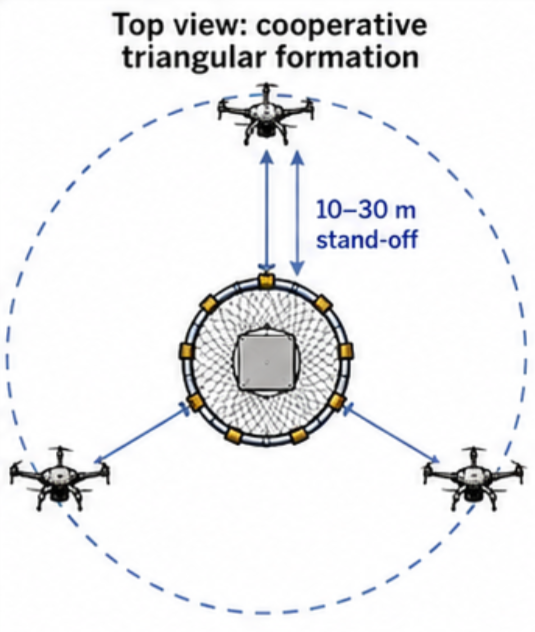
\includegraphics[width=0.33\textwidth]{figures/Concepts/conceptDtopview.png}
    \caption{Top-view conceptual layout of Concept D. Three cooperative UAVs remain connected to the payload-capture net through long tethers, allowing the formation to stabilise and steer the captured payload-net system during descent.}
    \label{fig:conceptD_topview}
\end{figure}

The interaction mechanism consists of a flexible HMPE/Dyneema payload net, a drawline closure system, distributed ballast modules, UAV-to-net tethers, and an optional backup parachute or parafoil. The net closes around the payload like a bag and mechanically locks after capture. The ballast is distributed around the net rim or lower net structure so that descent authority can be adjusted and partially released before landing.





\subsection{System Architecture}
\label{subsec:concept_D_architecture}

\subsubsection{Aerial Platform}

The aerial platform consists of three coordinated heavy-lift multirotor UAVs. The UAVs climb to the interception region, form a triangular formation below the target, and carry the payload-capture net through long stand-off tethers. A multirotor configuration is selected because the concept requires accurate hover, low-speed manoeuvring, and station keeping during payload capture.


\subsubsection{Sensing and Tracking}

% Initial target cueing is provided by the ground segment using radar, visual observation, or another external monitoring source. Once the UAV team reaches the search region, onboard EO/IR sensing is used for terminal tracking and formation alignment below the balloon-payload system.

                                                                                   

% In addition to the common target-tracking sensors, Concept D requires
% extra sensors for cooperative net control. The concept must control the
% relative motion of three UAVs, a suspended net, and a captured payload.

% First, ultra-wideband (UWB) ranging modules are considered between the three UAVs. These provide short-range relative distance measurements inside the formation and help maintain the triangular net geometry during capture and descent. This is specific to Concept D because the capture net position depends directly on the relative spacing between the UAVs, not only on each UAV's absolute GNSS position \cite{Shule2020UWB-BasedSurvey}.


% Second, inline tether tension sensors or compact load cells are considered at the UAV-to-net attachment points. These sensors measure the load in each tether and detect asymmetric loading, payload swing, or excessive tension before the formation becomes unstable. This is relevant for Concept D because the UAVs do not rigidly carry the payload, they steer and stabilise the suspended net through long tethers.  %\cite{Prkacin2025TrajectorySystems}.

% Third, a small IMU on the net rim or ballast frame is considered to estimate net attitude, net swing, and ballast-frame motion. This sensor is specific to Concept D because the net itself is an active part of the capture and descent dynamics. Without this measurement, the UAVs may know their own positions but not the orientation or oscillation state of the suspended net \cite{Sun2025AgileLoad,EstevezSanz2024ReviewQuadrotors}.

% Finally, visual markers or active LEDs on the net rim help each UAV
% estimate net shape and closure state using its onboard camera. These
% markers are useful because the flexible net may deform, twist, or close
% asymmetrically during capture.




% Initial target cueing is provided by the ground segment using radar, visual observation, or another external monitoring source. Once the UAV team reaches the search region, onboard EO/IR sensing is used for terminal tracking and formation alignment below the balloon-payload system. \\

                                                                                   

% In addition to the common target-tracking sensors, Concept D requires extra sensors that are specific to cooperative net control. These are not required to the same extent in the single-UAS or full-enclosure concepts because Concept D must control the relative motion of three UAVs, a suspended net, and a captured payload. \\

% First, ultra-wideband (UWB) ranging modules are considered between the three UAVs. These provide short-range relative distance measurements inside the formation and help maintain the triangular net geometry during capture and descent. This is specific to Concept D because the capture net position depends directly on the relative spacing between the UAVs, not only on each UAV's absolute GNSS position \cite{Shule2020UWB-BasedSurvey}. \\

% Second, inline tether tension sensors or compact load cells are considered at the UAV-to-net attachment points. These sensors measure the load in each tether and detect asymmetric loading, payload swing, or excessive tension before the formation becomes unstable. This is especially important for Concept D because the UAVs do not rigidly carry the payload; they steer and stabilise a suspended net through long flexible tethers \cite{Prkacin2025TrajectorySystems}.\\
 
% Third, a small IMU on the net rim or ballast frame is considered to estimate net attitude, net swing, and ballast-frame motion. This sensor is specific to Concept D because the net itself is an active part of the capture and descent dynamics. Without this measurement, the UAVs may know their own positions but not the orientation or oscillation state of the suspended net \cite{Sun2025AgileLoad,EstevezSanz2024ReviewQuadrotors}. \\

% Visual markers or active LEDs on the net rim may be considered to help each UAV estimate the net shape and closure state using its onboard camera. These markers are not required for concepts with a single rigid mechanism, but they are useful in Concept D because the flexible net may deform, twist or close asymmetrically during capture.

Concept D uses the common external-cueing architecture for initial target position, altitude, and drift estimation. Once near the target, onboard EO/IR sensing supports terminal tracking and formation alignment below the balloon-payload system. In addition to target tracking, Concept D requires cooperative-control sensing because the net position depends on the relative motion of three UAVs and a suspended flexible load. Ultra-wideband (UWB) ranging modules are included to estimate and maintain the relative spacing between the UAVs in the triangular formation \cite{Shule2020UWB-BasedSurvey}. Tether-tension sensors or compact load cells are included at the UAV-to-net attachment points to detect asymmetric loading, payload swing, or unsafe tether loads \cite{Prkacin2025TrajectorySystems}. The use of multiple UAVs to transport or stabilise a suspended load is supported by previous work on cooperative aerial manipulation and suspended-cable payload transport \cite{Sun2025AgileLoad,EstevezSanz2024ReviewQuadrotors}. A small IMU with visual markers or LEDs on the net rim is included as a concept-specific design feature to estimate net attitude, swing, deformation, and closure state.



\subsubsection{Balloon Interaction Mechanism}

The interaction mechanism consists of a flexible HMPE/Dyneema payload-capture net, a drawline closure system, distributed ballast modules, UAV-to-net tethers, and emergency release hardware. The net is positioned below the payload and then closed around it like a bag. A mechanical lock prevents reopening after capture. The system captures the payload or lower flight train rather than the balloon envelope itself, reducing the risk of uncontrolled rupture.





\subsubsection{Descent Initiation}

Descent is initiated by adding mass to the balloon-payload system. The attached net, ballast, tethers, and closure hardware must exceed the balloon residual free lift with sufficient margin:

\begin{equation}
    \left(m_{\mathrm{net}} + m_{\mathrm{ballast}} + m_{\mathrm{hardware}}\right)g 
    >
    B_{\mathrm{balloon}} - W_{\mathrm{payload}} + F_{\mathrm{margin}}
    \label{eq:ballast_descent_condition}
\end{equation}

where \(m_{\mathrm{net}}\) is the capture-net mass, \(m_{\mathrm{ballast}}\) is the ballast mass, \(m_{\mathrm{hardware}}\) includes tethers, closure devices, and release hardware, \(B_{\mathrm{balloon}}\) is the balloon buoyancy, \(W_{\mathrm{payload}}\) is the payload weight, and \(F_{\mathrm{margin}}\) is the required descent margin.

\subsubsection{Descent Management and Recovery}

During descent, the UAVs remain connected through long tethers and provide lateral steering toward the recovery zone. The descent rate is controlled mainly through the amount of ballast attached to the net. If the descent rate becomes too high near the ground, ballast can be released gradually. If tether loads become excessive or formation control is lost, an emergency parachute or parafoil can be deployed. After landing, the recovery crew retrieves the payload, net, ballast container, and reusable hardware.





% \subsection{Preliminary Mass and Cost Estimate}

% The cost estimate is based on catalogue-level component references and should therefore be interpreted as a prototype-level estimate, not a final procurement quotation. The table notes retain the main source basis for netting, tether line, cinch hardware, and the broad parachute/recovery-system cost range.
% \todo{this has to }
% \setlength{\tabcolsep}{3pt}

% \begin{longtable}{@{}
%     >{\raggedright\arraybackslash}p{0.2\textwidth}
%     >{\raggedright\arraybackslash}p{0.08\textwidth}
%     >{\raggedright\arraybackslash}p{0.1\textwidth}
%     >{\raggedright\arraybackslash}p{0.58\textwidth}
% @{}}

% \caption{Preliminary mass and cost estimate for the Concept D payload-capture hardware. Values exclude the three UAV platforms, onboard sensing hardware, batteries, and ground equipment.}
% \label{tab:conceptD_sizing_cost}\\

% \toprule
% \textbf{Item} & \textbf{Mass} & \textbf{Cost [EUR]} & \textbf{Basis / design relevance} \\
% \midrule
% \endfirsthead

% \caption[]{Preliminary mass and cost estimate for the Concept D payload-capture hardware. Continued.}\\
% \toprule
% \textbf{Item} & \textbf{Mass} & \textbf{Cost [EUR]} & \textbf{Basis / design relevance} \\
% \midrule
% \endhead

% \bottomrule
% \endfoot

% Payload capture net 
% & 2-5 kg 
% & 300-1500 
% & HMPE/Dyneema netting with reinforced rim and custom stitching. Catalogue netting is cheaper, but custom reinforcement and integration drive the estimate \cite{Netmark2026HMPE/DyneemaHM}. \\

% Tethers and attachments 
% & 0.3-1.0 kg 
% & 100-250 
% & Dyneema tether line, knots/splices, carabiners, and UAV-to-net attachment hardware \cite{Spearfishing.de2026DyneemaM}. \\

% Cinch and locking mechanism 
% & 0.5-1.5 kg 
% & 300-800 
% & Servo/winch, drum, guide rings, locking element, ESC/driver, and structural bracket. Catalogue servo-winch hardware gives the lower-bound reference \cite{FlashRC2026ServoTurns}. \\

% Granulated or liquid ballast modules 
% & 5-25 kg 
% & 50-300 
% & Sand, water, or another low-cost ballast plus pouches/containers. Cost is low, but mass is a major feasibility driver. \\

% Ballast and emergency release hardware 
% & 0.8--2.3 kg 
% & 300--900 
% & Release valves, cutters, small actuators, wiring, and redundant emergency release links. \\

% Backup parachute system 
% & 1-4 kg 
% & 1000-5000 
% & Emergency descent-rate reduction. The range covers simple prototype parachutes up to commercial UAV recovery systems \cite{MegaDron2026MOCSeries,UAVSystemsInternational2026DroneKg}. \\

% \midrule
% \textbf{Subtotal with backup parachute} 
% & \textbf{9.6-38.8 kg} 
% & \textbf{2050-8750} 
% & Prototype-level range for Concept D capture and descent hardware. \\

% UWB inter-UAV ranging modules
% & 0.1--0.3 kg
% & 300--900
% & Relative-position sensing between the three UAVs. Specific to Concept D because the net geometry depends on formation spacing \cite{Shule2020UWB-BasedSurvey}. \\

% Tether tension sensors / load cells
% & 0.2--0.6 kg
% & 300--1200
% & Measures load in each UAV-to-net tether and detects asymmetric loading, payload swing, or unsafe tension \cite{Prkacin2025TrajectorySystems}. \\

% Net/ballast-frame IMU and marker set
% & 0.1--0.4 kg
% & 100--500
% & Estimates net attitude and swing state; visual markers or LEDs help the UAVs observe net deformation and closure state. \\

% \end{longtable}



% As an off-the-shelf benchmark, a DJI FlyCart 30-class heavy-lift UAV is listed at approximately \(18{,}600~\mathrm{EUR}\) for the base aircraft and \(23{,}000{-}26{,}000~\mathrm{EUR}\) for more complete packages \cite{COPTERS.EU2026DJI30,DigitalAgro2026DJI30}. For three UAVs, this gives roughly \(69{,}000{-}77{,}000~\mathrm{EUR}\) for aircraft purchase alone. A custom UAV could reduce recurring cost, but would increase development, integration, and verification effort.


% For the climb-power estimate, the three UAVs are assumed to carry \(30~\mathrm{kg}\) of Concept-D payload in total, or \(10~\mathrm{kg}\) per UAV. With a fixed non-battery mass of \(22~\mathrm{kg}\) per UAV, the refined estimate gives a battery mass of \(19.79~\mathrm{kg}\) and an MTOW of \(41.79~\mathrm{kg}\) per UAV. A \(5~\mathrm{m/s}\) climb rate is used because the FlyCart 30 lists this ascent speed with a \(30~\mathrm{kg}\) payload under zero-altitude, windless conditions, while its \(6000~\mathrm{m}\) altitude capability is only listed for the no-payload case \cite{DJI2026DJISpecifications}. A \(10~\mathrm{m/s}\) climb rate is therefore rejected for this concept, especially since multirotor ascent power increases with climb speed and reduced air density \cite{DJI2026DJISpecificationsd,Gong2022ModellingUAVs}.


% % As a commercial off-the-shelf reference, the DJI FlyCart 30 gives an indicative purchase price for a heavy-lift UAV in this class. Public European listings place the base FlyCart 30 at approximately \(18{,}600~\mathrm{EUR}\), while more complete packages including key operating hardware are listed at approximately \(23{,}000{-}26{,}000~\mathrm{EUR}\) per UAV \cite{COPTERS.EU2026DJI30,DigitalAgro2026DJI30}. For a three-UAV Concept D architecture, this would correspond to roughly \(69{,}000{-}77{,}000~\mathrm{EUR}\) for the aircraft purchase alone, excluding mission-specific nets, tethers, recovery hardware, integration, testing, spares, and additional batteries. This value should therefore be interpreted as an off-the-shelf procurement benchmark rather than the expected final production cost. A custom UAV developed from selected components would likely reduce the recurring unit cost, but would require substantially more design, manufacturing, integration, verification, and testing effort, increasing development time and project resource demand.



% % For the climb-power estimate, the three UAVs are assumed to jointly carry a maximum Concept-D payload of \(30~\mathrm{kg}\), giving \(10~\mathrm{kg}\) per UAV. A fixed non-battery mass of \(22~\mathrm{kg}\) per UAV is assumed, consisting of \(12~\mathrm{kg}\) vehicle mass and \(10~\mathrm{kg}\) payload share. The refined battery sizing gives a battery mass of \(19.79~\mathrm{kg}\) per UAV, resulting in an estimated MTOW of \(41.79~\mathrm{kg}\) per UAV.

% % The closest publicly available heavy-lift multirotor reference is the DJI FlyCart 30. It can carry a \(30~\mathrm{kg}\) payload in dual-battery mode and lists a maximum ascent speed of \(5~\mathrm{m/s}\) with this payload under zero-altitude, windless test conditions. However, its \(6000~\mathrm{m}\) maximum flight altitude is listed only for the no-payload case, so a loaded climb to \(6000~\mathrm{m}\) is already an optimistic assumption \cite{DJI2026DJISpecifications}. A \(10~\mathrm{m/s}\) climb rate is therefore rejected for Concept D sizing, even though smaller enterprise UAVs can reach this value with much lower payload capacity \cite{DJI2026DJISpecificationsd}. Multirotor power-consumption studies also show that vertical-ascent power is higher than hover power and increases with ascent speed \cite{Gong2022ModellingUAVs}.

% The battery sizing uses a source-anchored power-loading method. From the DJI FlyCart 30 battery energy and hover endurance, the sea-level hover benchmark is approximately \(139~\mathrm{W/kg}\). To account for vertical climb, reduced air density at \(6000~\mathrm{m}\), suspended hardware, and preliminary uncertainty, the refined Concept D estimate uses an average climb power of \(8.63~\mathrm{kW}\) per UAV, corresponding to approximately \(206~\mathrm{W/kg}\) on the estimated MTOW. The resulting mission energy consumption is \(3.48~\mathrm{kWh}\) per UAV, including the \(3~\mathrm{min}\) terminal hover/capture allowance and \(10\%\) energy contingency. With a \(20\%\) unusable battery reserve, the installed battery energy is \(4.35~\mathrm{kWh}\) per UAV. Using a battery specific energy of \(220~\mathrm{Wh/kg}\), this gives a required battery mass of \(19.79~\mathrm{kg}\) per UAV.


% \begin{table}[H]
% \centering
% \small
% \caption{Concept D battery-mass estimate for a $5~\mathrm{m/s}$ climb to $6000~\mathrm{m}$, including $3~\mathrm{min}$ terminal hover, $10\%$ energy contingency, and $20\%$ battery reserve.}
% \label{tab:conceptD_battery_mass_estimate}
% \setlength{\tabcolsep}{3pt} % Reduced padding to save horizontal space
% \renewcommand{\arraystretch}{1.3}
% \begin{tabular}{
%     >{\centering\arraybackslash}p{0.14\linewidth}
%     >{\centering\arraybackslash}p{0.12\linewidth}
%     >{\centering\arraybackslash}p{0.12\linewidth}
%     >{\centering\arraybackslash}p{0.15\linewidth}
%     >{\centering\arraybackslash}p{0.12\linewidth}
%     >{\centering\arraybackslash}p{0.15\linewidth}
%     >{\centering\arraybackslash}p{0.10\linewidth}
% }
% \toprule
% \textbf{Battery specific energy} & 
% \textbf{Battery per UAV} & 
% \textbf{MTOW per UAV} & 
% \textbf{Avg. climb power per UAV} & 
% \textbf{Mission energy per UAV} & 
% \textbf{Installed battery energy} & 
% \textbf{Team battery mass} \\
% \midrule
% $220~\mathrm{Wh/kg}$ & $19.79~\mathrm{kg}$ & $41.79~\mathrm{kg}$ & $8.63~\mathrm{kW}$ & $3.48~\mathrm{kWh}$ & $4.35~\mathrm{kWh}$ & $59.37~\mathrm{kg}$ \\
% \bottomrule
% \end{tabular}
% \end{table}


% Using the shared descent-rate estimate in Section~\ref{sec:shared_descent_rate_estimate}, a \(6~\mathrm{m}\) balloon with \(10\)--\(15~\mathrm{kg}\) of excess downward mass descends in approximately \(20\)--\(24~\mathrm{min}\). This is acceptable from a descent-rate safety perspective, but increases horizontal drift and makes recovery-zone accuracy dependent on wind, tether steering authority, and possible parachute or parafoil support.

% The approximate direct-climb mission time is therefore \(20~\mathrm{min}\) for climb, \(3~\mathrm{min}\) for terminal formation and capture, and \(20\)--\(24~\mathrm{min}\) for descent in the large-balloon case. A sequential \(6~\mathrm{km}\) horizontal transit at \(15~\mathrm{m/s}\) would add approximately \(6.7~\mathrm{min}\), although climb and translation may occur simultaneously.

% Overall, Concept D is attractive because it avoids destructive balloon-envelope interaction, but it is weak as a direct high-altitude interception architecture. It should therefore be penalised in the trade-off unless combined with a carrier aircraft, pre-positioned airborne loiter, or a lower operational altitude envelope.




% % The descent behaviour of Concept D is assessed using the shared descent-rate estimate in Section~\ref{sec:shared_descent_rate_estimate}. For the large-balloon case, Table~\ref{tab:shared_descent_time_estimate} indicates that a \(6~\mathrm{m}\) balloon with \(10\)--\(15~\mathrm{kg}\) of excess downward mass would descend in approximately \(20\)--\(24~\mathrm{min}\). This is acceptable from a descent-rate safety perspective, but it increases horizontal drift and makes recovery-zone accuracy dependent on wind, tether steering authority, and possible parachute or parafoil support.

% % The approximate direct-climb time budget for Concept D is therefore \(20~\mathrm{min}\) for climb, \(3~\mathrm{min}\) for terminal formation and capture, and approximately \(20\)--\(24~\mathrm{min}\) for descent in the large-balloon case. Horizontal transit is not included because climb and translation may occur simultaneously; if performed sequentially, a \(6~\mathrm{km}\) horizontal transit at \(15~\mathrm{m/s}\) adds approximately \(6.7~\mathrm{min}\).

% % Overall, Concept D remains attractive because it avoids destructive balloon-envelope interaction, but it is weak as a direct high-altitude interception architecture. It should be penalised in the trade-off unless combined with a carrier aircraft, pre-positioned airborne loiter, or a lower operational altitude envelope.






% \subsection{Preliminary Mass and Cost Estimate}
% The estimate is based on catalogue-level component references and should be interpreted as a prototype-level estimate, not a final procurement quotation. The net mass and cost use HMPE/Dyneema catalogue netting as a lower-bound reference, while the reinforced rim, stitching, and integration margin are internal design estimates \cite{Netmark2026HMPE/DyneemaHM}. The tether estimate uses a 2 mm Dyneema line as the catalogue reference; knots, splices, carabiners, and UAV-to-net attachment hardware are added as engineering allowances \cite{Spearfishing.de2026DyneemaM}. The cinch and locking mechanism uses servo/winch-type hardware as a lower-bound catalogue reference, while the drum, guide rings, locking element, driver, and structural bracket are added as integration allowances \cite{FlashRC2026ServoTurns}. The backup parachute or parafoil range is bounded using available UAV recovery-system examples rather than a final Concept-D-specific recovery system \cite{MegaDron2026MOCSeries,UAVSystemsInternational2026DroneKg}. The values in Table~\ref{tab:conceptD_sizing_cost} exclude the three UAV platforms, batteries, ground equipment, integration, testing, spares, and additional batteries.

% \begin{table}[H]
% \centering
% \small
% \caption{Preliminary mass and cost estimate for Concept D mission-specific hardware.}
% \label{tab:conceptD_sizing_cost}
% \setlength{\tabcolsep}{6pt}
% \renewcommand{\arraystretch}{1.18}
% \begin{tabularx}{0.82\textwidth}{@{}Xcc@{}}
% \toprule
% \textbf{Item} & \textbf{Mass [kg]} & \textbf{Cost [EUR]} \\
% \midrule
% Payload-capture net & 2--5 & 300--1500 \\
% Tethers and attachments & 0.3--1.0 & 100--250 \\
% Cinch and locking mechanism & 0.5--1.5 & 300--800 \\
% Ballast modules & 5--25 & 50--300 \\
% Ballast and emergency release hardware & 0.8--2.3 & 300--900 \\
% Backup parachute/parafoil & 1--4 & 1000--5000 \\
% Cooperative-control sensors & 0.4--1.3 & 700--2600 \\
% \midrule
% \textbf{Total, excluding UAVs} & \textbf{10.0--40.1} & \textbf{2750--11350} \\
% \bottomrule
% \end{tabularx}
% \end{table}
% The cooperative-control sensor package includes UWB inter-UAV ranging modules, tether-tension sensors or compact load cells, and a net/ballast-frame IMU with visual markers or LEDs. UWB ranging is included because the net geometry depends on the relative spacing between the three UAVs \cite{Shule2020UWB-BasedSurvey}. Tether-tension sensing is included because the UAVs act on the net through flexible tethers, so asymmetric loading, payload swing, or excessive tether loads must be detected before the formation becomes unstable \cite{Prkacin2025TrajectorySystems}. The IMU and visual markers are included as concept-specific design choices to estimate net attitude, swing, deformation, and closure state.
% As an off-the-shelf benchmark, a DJI FlyCart 30-class heavy-lift UAV is used to estimate the order of magnitude of the aircraft procurement cost. Public European listings place the base aircraft at approximately \(18{,}600~\mathrm{EUR}\) \cite{COPTERS.EU2026DJI30}, while more complete packages are listed at approximately \(23{,}000{-}26{,}000~\mathrm{EUR}\) per UAV \cite{DigitalAgro2026DJI30}. For three UAVs, this gives roughly \(69{,}000{-}77{,}000~\mathrm{EUR}\) for aircraft purchase alone. A custom UAV could reduce recurring unit cost, but would increase development, integration, verification, and testing effort.


\subsection{Preliminary Mass and Cost Estimate}

The estimate is based on catalogue-level component references and should be interpreted as a prototype-level estimate, not a final procurement quotation. The net mass and cost use HMPE/Dyneema catalogue netting as a lower-bound reference, while the reinforced rim, stitching, and integration margin are internal design estimates \cite{Netmark2026HMPE/DyneemaHM}. The tether estimate uses a 2 mm Dyneema line as the catalogue reference; knots, splices, carabiners, and UAV-to-net attachment hardware are added as engineering allowances \cite{Spearfishing.de2026DyneemaM}. The cinch and locking mechanism uses servo/winch-type hardware as a lower-bound catalogue reference, while the drum, guide rings, locking element, driver, and structural bracket are added as integration allowances \cite{FlashRC2026ServoTurns}. The backup parachute or parafoil range is bounded using available UAV recovery-system examples rather than a final Concept-D-specific recovery system \cite{MegaDron2026MOCSeries,UAVSystemsInternational2026DroneKg}.

\begin{table}[H]
\centering
\small
\caption{Preliminary mass and cost estimate for Concept D. Mission-specific hardware is separated from the COTS heavy-lift UAV procurement benchmark.}
\label{tab:conceptD_sizing_cost}
\setlength{\tabcolsep}{5pt}
\renewcommand{\arraystretch}{1.18}
\begin{tabularx}{0.95\textwidth}{@{}Xcc@{}}
\toprule
\textbf{Item} & \textbf{Mass [kg]} & \textbf{Cost [EUR]} \\
\midrule
Payload-capture net & 2--5 & 300--1500 \\
Tethers and attachments & 0.3--1.0 & 100--250 \\
Cinch and locking mechanism & 0.5--1.5 & 300--800 \\
Ballast modules & 5--25 & 50--300 \\
Ballast and emergency release hardware & 0.8--2.3 & 300--900 \\
Backup parachute/parafoil & 1--4 & 1000--5000 \\
Cooperative-control sensors & 0.4--1.3 & 700--2600 \\
\midrule
\textbf{Subtotal, mission-specific hardware} & \textbf{10.0--40.1} & \textbf{2750--11350} \\
\midrule
COTS heavy-lift UAV procurement benchmark, three vehicles & -- & 69000--78000 \\
\midrule
\textbf{Indicative total hardware acquisition cost} & -- & \textbf{71750--89350} \\
\bottomrule
\end{tabularx}
\end{table}

The cooperative-control sensor package includes UWB inter-UAV ranging modules, tether-tension sensors or compact load cells, and a net/ballast-frame IMU with visual markers or LEDs. UWB ranging is included because the net geometry depends on the relative spacing between the three UAVs \cite{Shule2020UWB-BasedSurvey}. Tether-tension sensing is included because the UAVs act on the net through flexible tethers, so asymmetric loading, payload swing, or excessive tether loads must be detected before the formation becomes unstable \cite{Prkacin2025TrajectorySystems}. The IMU and visual markers are included as concept-specific design choices to estimate net attitude, swing, deformation, and closure state. \\ \\

As an off-the-shelf benchmark, a DJI FlyCart 30-class heavy-lift UAV is used to estimate the order of magnitude of the aircraft procurement cost. Public European listings place the base aircraft at approximately \(18{,}600~\mathrm{EUR}\) \cite{COPTERS.EU2026DJI30}, while more complete packages are listed at approximately \(23{,}000{-}26{,}000~\mathrm{EUR}\) per UAV \cite{DigitalAgro2026DJI30}. For three UAVs, this gives roughly \(69{,}000{-}78{,}000~\mathrm{EUR}\) for aircraft procurement alone. Combining this benchmark with the mission-specific hardware gives an indicative total hardware acquisition cost of approximately \(71{,}750{-}89{,}350~\mathrm{EUR}\). This total excludes ground equipment, integration, testing, spares, and additional batteries. A custom UAV could reduce recurring unit cost, but would increase development, integration, verification, and testing effort. \\ \\

For the climb-power estimate, the three UAVs are assumed to carry \(30~\mathrm{kg}\) of Concept-D payload in total. With a fixed non-battery mass of \(22~\mathrm{kg}\) per UAV, the refined estimate gives a battery mass of \(19.79~\mathrm{kg}\) and an MTOW of \(41.79~\mathrm{kg}\) per UAV. A \(5~\mathrm{m/s}\) climb rate is used because the FlyCart 30 lists this ascent speed with a \(30~\mathrm{kg}\) payload under zero-altitude, windless test conditions \cite{DJI2026DJISpecifications}. However, the same specifications list the \(6000~\mathrm{m}\) altitude capability only for the no-payload case, so loaded climb to \(6000~\mathrm{m}\) remains an optimistic assumption \cite{DJI2026DJISpecifications}. A \(10~\mathrm{m/s}\) climb rate is rejected for Concept D because comparable UAVs with this higher ascent speed have much lower payload capacity. This choice is also consistent with multirotor power-consumption modelling, which shows that vertical-ascent power increases with climb speed \cite{Gong2022ModellingUAVs}.


% 
\begin{table}[H]
\centering
\small
\caption{Concept D battery estimate for a $5~\mathrm{m/s}$ climb to $6000~\mathrm{m}$.}
\label{tab:conceptD_battery_mass_estimate}
\setlength{\tabcolsep}{5pt}
\renewcommand{\arraystretch}{1.18}
\begin{tabularx}{0.9\textwidth}{@{}XXXXX@{}}
\toprule
\textbf{Battery specific energy} & 
\textbf{Battery per UAV} & 
\textbf{MTOW per UAV} & 
\textbf{Mission energy per UAV} & 
\textbf{Team battery mass} \\
\midrule
$220~\mathrm{Wh/kg}$ & $19.79~\mathrm{kg}$ & $41.79~\mathrm{kg}$ & $3.48~\mathrm{kWh}$ & $59.37~\mathrm{kg}$ \\
\bottomrule
\end{tabularx}
\end{table}

Using the descent-rate estimates, a \(6~\mathrm{m}\) balloon with \(10\)--\(15~\mathrm{kg}\) of excess downward mass descends in approximately \(20\)--\(24~\mathrm{min}\). This is acceptable from a descent-rate safety perspective, but it increases horizontal drift and makes recovery-zone accuracy dependent on wind, tether steering authority, and possible parachute or parafoil support. \\

The approximate direct-climb mission time is therefore \(20~\mathrm{min}\) for climb, \(3~\mathrm{min}\) for terminal formation and capture, and \(20\)--\(24~\mathrm{min}\) for descent in the large-balloon case. A sequential \(6~\mathrm{km}\) horizontal transit at \(15~\mathrm{m/s}\) would add approximately \(6.7~\mathrm{min}\), although climb and translation may occur simultaneously.\\

Overall, Concept D is attractive because it avoids destructive balloon-envelope interaction, but it is weak as a direct high-altitude interception architecture. It should therefore be penalised in the trade-off unless combined with a carrier aircraft, pre-positioned airborne loiter, or a lower operational altitude envelope.\\







\subsection{Risks and Uncertainties}

{
\small
\setlength{\LTleft}{0pt}
\setlength{\LTright}{0pt}

\begin{longtable}{@{}p{0.20\textwidth} p{0.4\textwidth} p{0.35\textwidth}@{}}
\caption{Key risks for the cooperative variable-weight payload net concept.}
\label{tab:conceptD_key_risks} \\
\toprule
\textbf{Risk} & \textbf{Effect on mission} & \textbf{Possible mitigation} \\
\midrule
\endfirsthead

\toprule
\textbf{Risk} & \textbf{Effect on mission} & \textbf{Possible mitigation} \\
\midrule
\endhead

\bottomrule
\endfoot

Required ballast mass is too high & UAVs cannot carry or control the net, making the concept infeasible for high-buoyancy targets. & Include a go/no-go check based on estimated residual free lift. \\
Battery mass is too high & Direct climb to \(6000~\mathrm{m}\) becomes impractical or exceeds the response-time requirement. & Use carrier aircraft, pre-positioned loiter, or lower operational altitude envelope. \\
Payload capture fails & Mission fails before descent initiation. & Increase net aperture, improve payload tracking, and allow multiple capture attempts. \\
Tether or formation instability & UAVs may lose control or the payload may swing unpredictably. & Use long stand-off tethers, tension monitoring, and emergency release hardware. \\
Uncontrolled or hard landing & Payload, net, or ground area may be damaged. & Use controlled ballast release and backup parachute/parafoil deployment. \\

\end{longtable}
}





% Concept D provides a cooperative, non-destructive recovery architecture in which three heavy-lift multirotors carry and stabilise a flexible HMPE/Dyneema net around the payload or lower flight train. Its main advantage is that it avoids direct balloon-envelope damage while allowing ballast-based descent control and possible recovery of the payload and hardware. However, the concept is strongly limited by ballast mass, battery mass, formation-control complexity, tether-load uncertainty, and poor feasibility for direct high-altitude interception. It is therefore most suitable for moderate-altitude recovery or for operation with a carrier/loiter platform, and should be penalised for direct high-altitude interception.





